\documentclass[a4paper,oneside,12pt]{report}
% Package yang diperlukan
\usepackage{fontspec}       % Font sistem untuk XeLaTeX
\usepackage{setspace}       % Pengaturan jarak antarbaris
\usepackage{graphicx}      % Untuk memasukkan gambar
\usepackage{titling}       % Untuk kustomisasi halaman judul
\usepackage{geometry}      % Untuk mengatur margin halaman
\usepackage{listings}      % Untuk menampilkan blok kode
\usepackage{xcolor}        % Untuk menggunakan warna
\usepackage{float}         % Untuk kontrol penempatan float
\usepackage{xurl}          % Untuk pemutusan tautan URL yang lebih baik
\usepackage{hyperref}      % Untuk membuat hyperlink (URL, referensi)
\usepackage{indentfirst}   % Indentasi paragraf pertama setiap seksi
\usepackage{url}           % Format URL
\usepackage{fancyhdr}      % Header dan footer
\usepackage{tocloft}       % Kustomisasi Daftar Isi
\usepackage{bookmark}      % Manajemen bookmark PDF
\usepackage{amsmath}       % Rumus matematika
\usepackage{amssymb}       % Simbol matematika
\usepackage{booktabs}      % Tabel rapi
\usepackage{caption}
\usepackage{subcaption}    % Gambar berdampingan
\usepackage{tabularx}      % Tabel lebar otomatis
\usepackage{array}         % Kontrol kolom tabel
\usepackage{enumitem}      % Kontrol kerapatan daftar
\usepackage[none]{hyphenat} % Nonaktifkan pemotongan kata bertanda hubung
\usepackage{microtype}     % Tipografi halus dan protrusion

% Font dan spasi standar laporan praktikum
\setmainfont{Times New Roman}
\onehalfspacing

%======================================================================
% PENGATURAN GEOMETRI HALAMAN
%======================================================================
\geometry{left=3cm, right=2.5cm, top=2cm, bottom=2.5cm}
\sloppy
\tolerance=10000
\emergencystretch=3em
\hfuzz=1.5pt
\hbadness=10000
\hyphenpenalty=10000
\exhyphenpenalty=10000
\righthyphenmin=62
\lefthyphenmin=62

%======================================================================
% PENGATURAN WARNA BLOK KODE
%======================================================================
\definecolor{codegreen}{rgb}{0,0.6,0}
\definecolor{codegray}{rgb}{0.5,0.5,0.5}
\definecolor{codepurple}{rgb}{0.58,0,0.82}
\definecolor{backcolour}{rgb}{0.95,0.95,0.92}
\definecolor{darkblue}{rgb}{0,0,0.6}

\lstdefinestyle{commonstyle}{
    backgroundcolor=\color{backcolour},
    breakatwhitespace=false,
    breaklines=true,
    captionpos=b,
    keepspaces=true,
    numbers=left,
    numbersep=5pt,
    showspaces=false,
    showstringspaces=false,
    showtabs=false,
    tabsize=2,
    frame=single,
    basicstyle=\ttfamily\scriptsize,
    numberstyle=\tiny\color{codegray},
    columns=flexible,
    postbreak=\mbox{\textcolor{red}{$\hookrightarrow$}\space},
    breakindent=0pt,
    breakautoindent=false
}

\lstdefinestyle{pythonstyle}{
    style=commonstyle,
    language=Python,
    commentstyle=\color{codegreen},
    keywordstyle=\color{darkblue},
    stringstyle=\color{codepurple},
    emph={import,from,class,def,for,while,if,else,elif,try,except,finally,with,as,return},
    emphstyle=\color{darkblue}
}

\lstdefinestyle{bashstyle}{
    style=commonstyle,
    language=bash,
    numbers=none,
    commentstyle=\color{codegreen},
    keywordstyle=\color{black},
    stringstyle=\color{codepurple}
}

%======================================================================
% PENGATURAN LAIN-LAIN
%======================================================================
\newcommand{\customfbox}[1]{%
  \setlength{\fboxsep}{0pt}%
  \setlength{\fboxrule}{0.5pt}%
  \fcolorbox{black}{white}{#1}%
}
\renewcommand{\figurename}{Gambar}
\renewcommand{\thefigure}{\arabic{figure}}
\renewcommand{\tablename}{Tabel}
\renewcommand{\thetable}{\arabic{table}}
\renewcommand{\theequation}{\arabic{equation}}
\renewcommand{\lstlistingname}{Listing}
\AtBeginDocument{\renewcommand{\thelstlisting}{\arabic{lstlisting}}}
\counterwithout{figure}{chapter}
\counterwithout{table}{chapter}
\counterwithout{equation}{chapter}

\hypersetup{
    colorlinks=true,
    linkcolor=black,
    filecolor=black,
    urlcolor=black,
    citecolor=black,
    pdftitle={Laporan Praktikum Penambangan Data Pertemuan 11 - Model Deployment (Flask dan Streamlit)},
    pdfpagemode=FullScreen,
    breaklinks=true
}

\pagestyle{fancy}
\fancyhf{}
\fancyfoot[C]{\thepage}
\renewcommand{\headrulewidth}{0pt}
\fancypagestyle{plain}{
    \fancyhf{}
    \fancyfoot[C]{\thepage}
    \renewcommand{\headrulewidth}{0pt}
}

\makeatletter
\renewcommand{\@makechapterhead}[1]{%
  {\parindent\z@ \raggedright \normalfont \Huge\bfseries #1\par\nobreak \vskip 24\p@}}
\renewcommand{\@makeschapterhead}[1]{%
  {\parindent\z@ \raggedright \normalfont \Huge\bfseries #1\par\nobreak \vskip 24\p@}}
\makeatother

\renewcommand{\contentsname}{Daftar Isi}
\renewcommand{\bibname}{Daftar Pustaka}
\renewcommand{\thechapter}{}
\renewcommand{\chaptername}{}
\renewcommand{\thesection}{\arabic{chapter}.\arabic{section}}
\renewcommand{\thesubsection}{\thesection.\arabic{subsection}}
\setcounter{secnumdepth}{3}
\setcounter{tocdepth}{3}

\renewcommand{\cftchapdotsep}{\cftdotsep}
\renewcommand{\cftchapleader}{\cftdotfill{\cftchapdotsep}}
\setlength{\cftchapindent}{0em}
\setlength{\cftsecindent}{2em}
\setlength{\cftsubsecindent}{4em}
\setlength{\cftchapnumwidth}{0em}
\setlength{\cftsecnumwidth}{2.5em}
\setlength{\cftsubsecnumwidth}{3.2em}
\setlength{\cftbeforechapskip}{4pt}
\setlength{\cftbeforesecskip}{1.5pt}
\setlength{\cftbeforesubsecskip}{0.5pt}
\renewcommand{\cftchappresnum}{}
\renewcommand{\cftchapaftersnum}{}
\newcommand{\tocboldsection}[1]{%
  \protect\renewcommand{\protect\cftchapfont}{\protect\bfseries}%
  #1%
  \protect\renewcommand{\protect\cftchapfont}{}%
}

%======================================================================
% AWAL DOKUMEN
%======================================================================
\begin{document}

% Halaman Judul
\newgeometry{left=3cm, right=2.5cm, top=2.5cm, bottom=3cm}
\begin{titlingpage}
	\begin{spacing}{1}
		\begin{center}
			\vspace*{0.2cm}
			{\large \textbf{\MakeUppercase{Laporan Praktikum}}} \\[0.4cm]
			{\large \textbf{\MakeUppercase{Praktikum Penambangan Data}}} \\[0.4cm]
			{\large \textbf{\MakeUppercase{Pertemuan 11}}} \\[0.4cm]
			{\large \textbf{\MakeUppercase{Model Deployment (Flask dan Streamlit)}}} \\[1.5cm]

			
\includegraphics[height=7cm]{images/UGM.png} \\[0.7cm]

			{\normalsize \textbf{Disusun oleh:}} \\[0.4cm]
			\begin{tabular}{@{}l l @{}}
				\textbf{Nama}           & : Hafidz Rizqullah Prasetya        \\
				\textbf{NIM}            & : 24/535493/SV/24243               \\
				\textbf{Kelas}          & : PL5A1                            \\
				\textbf{Dosen Pengampu} & : Dr. Imam Fahrurrozi, S.T., M.Cs.
			\end{tabular} \\[1.2cm]

			{\normalsize \textbf{PROGRAM STUDI D-IV}} \\[0.2cm]
			{\normalsize \textbf{TEKNOLOGI REKAYASA PERANGKAT LUNAK}} \\[0.2cm]
			{\normalsize \textbf{DEPARTEMEN TEKNIK ELEKTRO DAN INFORMATIKA}} \\[0.2cm]
			{\normalsize \textbf{SEKOLAH VOKASI}} \\[0.2cm]
			{\normalsize \textbf{UNIVERSITAS GADJAH MADA}} \\[0.2cm]
			{\normalsize \textbf{YOGYAKARTA}} \\[0.2cm]
			{\normalsize \textbf{2026}} \\[1.2cm]
		\end{center}
	\end{spacing}
\end{titlingpage}
\restoregeometry

\thispagestyle{empty}
\clearpage
\stepcounter{page}
\thispagestyle{empty}

% --- Daftar Isi ---
\addcontentsline{toc}{chapter}{Daftar Isi}
\begin{spacing}{0.92}
	\tableofcontents
\end{spacing}
\clearpage

% Penomoran halaman Arab mulai dari 3
\pagenumbering{arabic}
\setcounter{page}{3}

\chapter[Tujuan Praktikum]{Tujuan Praktikum}
Berdasarkan Modul Praktikum Penambangan Data Pertemuan X dan XI serta silabus pembelajaran, tujuan praktikum ini adalah:
\begin{enumerate}[noitemsep, topsep=4pt, parsep=2pt]
	\item Memahami konsep dasar dan urgensi \textit{model deployment} dalam siklus hidup penambangan data (\textit{Machine Learning Lifecycle}).
	\item Melakukan proses \textit{serialization} (penyimpanan biner) dan \textit{deserialization} (pemuatan kembali) model \textit{machine learning} terlatih menggunakan pustaka \texttt{joblib} dan \texttt{pickle}.
	\item Memahami perbedaan paradigma arsitektur antara layanan web berbasis RESTful API (\textit{client-server request-response} pada Flask) dan aplikasi analitik data reaktif (\textit{script re-run execution} pada Streamlit).
	\item Membangun layanan \textit{web service} sederhana dengan \textit{micro-framework} Flask untuk menyajikan inferensi prediksi model melalui protokol HTTP (metode GET dan POST) serta antarmuka formulir HTML.
	\item Membangun aplikasi web dan \textit{dashboard} data interaktif menggunakan framework Streamlit tanpa memerlukan kode \textit{front-end} (HTML/CSS/JavaScript) terpisah.
	\item Menerapkan mekanisme optimasi performa melalui \textit{caching} (\texttt{@st.cache\_resource} dan \texttt{@st.cache\_data}) serta pengelolaan status antarmuka (\textit{Session State}) pada Streamlit.
	\item Mengintegrasikan model \textit{Decision Tree} (dataset Hepatitis C) dan model \textit{Support Vector Machine} terkalibrasi dari proyek GlucoSense (dataset risiko diabetes) ke dalam layanan Flask dan antarmuka Streamlit.
	\item Melakukan analisis perbandingan komparatif antara Flask dan Streamlit dari aspek arsitektur, kecepatan pengembangan, latensi inferensi, dan skenario penerapan industri.
\end{enumerate}

\clearpage

\chapter{Dasar Teori}

\section{Model Deployment dalam Siklus Hidup Machine Learning}
Pengembangan sistem berbasis \textit{machine learning} bukanlah proses sekali jalan, melainkan sebuah siklus terstruktur yang dikenal sebagai \textit{Machine Learning Lifecycle} atau metodologi CRISP-DM \cite{han2022}. Tahapan komprehensif ini meliputi perumusan masalah (\textit{problem definition}), pengumpulan data, prapemrosesan data, eksplorasi data analitis (EDA), rekayasa fitur, pelatihan model, serta evaluasi dan penalaan hiperparameter. Hingga tahap evaluasi, model yang dihasilkan masih berada di lingkungan komputasi pengembang (\textit{Jupyter Notebook} atau skrip Python lokal).

\begin{figure}[H]
	\centering
	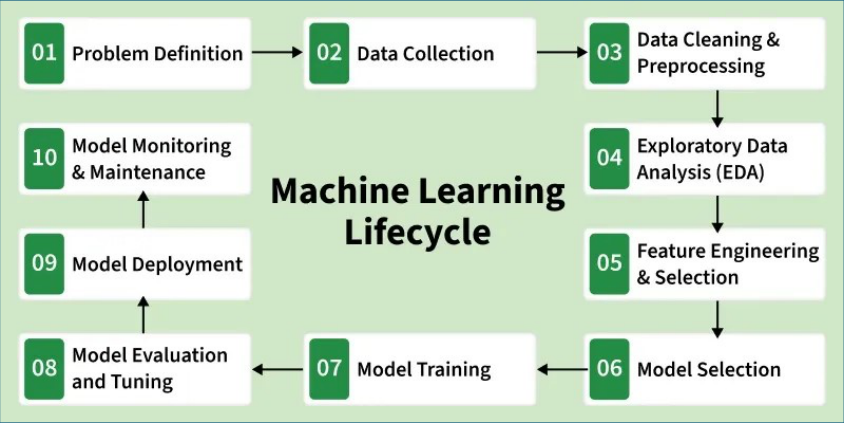
\includegraphics[width=0.72\textwidth]{images/gambar-10-2-1-machine-learning-lifecycle-sumber-www-geeksforgeeks-org.png}
	\caption{Siklus Hidup Pengembangan Machine Learning (ML Lifecycle).}
	\label{fig:teori-lifecycle}
\end{figure}

Model yang hanya tersimpan di dalam memori \textit{notebook} tidak dapat dimanfaatkan secara praktis oleh pengguna akhir maupun diintegrasikan ke sistem perangkat lunak lain. \textit{Model deployment} mentransformasikan objek model statis menjadi sebuah layanan komputasi aktif yang dapat menerima data masukan baru dan menghasilkan inferensi prediksi secara andal \cite{treveil2020}. Skema umum \textit{deployment} terdiri atas \textit{embedded model} (tertanam langsung pada perangkat/klien), \textit{batch prediction} (prediksi berkala terhadap kumpulan data dalam jumlah besar), dan arsitektur \textit{client-server} berbasis antarmuka web atau RESTful API.

\section{Arsitektur Client-Server dan Metode HTTP}
Pada arsitektur \textit{client-server}, model inferensi berjalan pada lingkungan server komputasi terpusat, sementara klien (peramban web, aplikasi seluler, atau sistem pihak ketiga) berkomunikasi melalui jaringan memanfaatkan protokol HTTP \cite{fielding2000}.

\begin{figure}[H]
	\centering
	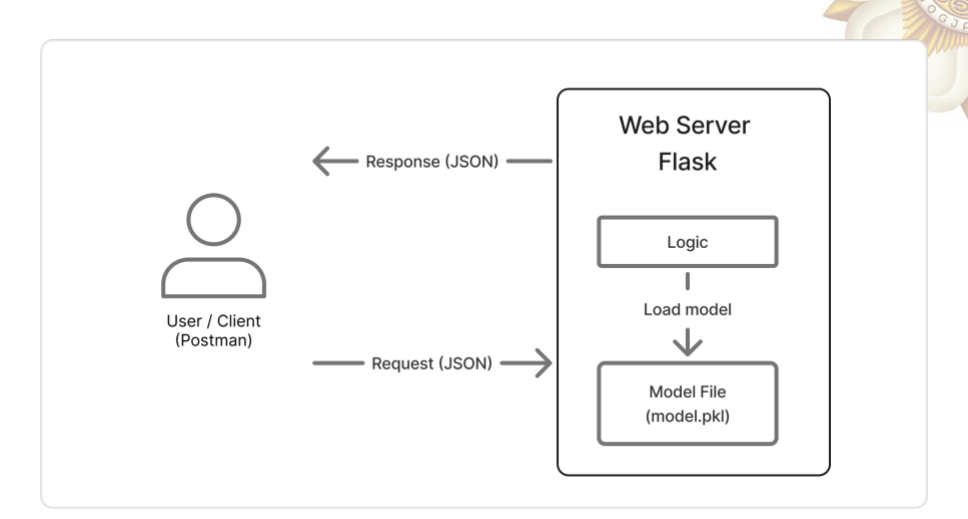
\includegraphics[width=0.75\textwidth]{images/gambar-10-2-2-skema-alur-data-client-server.png}
	\caption{Skema Alur Pertukaran Data Client-Server untuk Inferensi Model.}
	\label{fig:teori-clientserver}
\end{figure}

Alur inferensi data pada arsitektur \textit{client-server} terdiri dari lima tahapan berurutan:
\begin{enumerate}[noitemsep, topsep=3pt, parsep=2pt]
	\item Klien mengakses alamat URL (\textit{endpoint}) yang disediakan server web.
	\item Klien mengirimkan nilai fitur masukan melalui formulir web (\textit{form data}) atau muatan JSON (\textit{payload}) menggunakan metode HTTP POST.
	\item Pengontrol server (\textit{controller}) melakukan penguraian (\textit{parsing}), validasi tipe data, dan transformasi struktur matriks masukan agar sesuai dengan spesifikasi dimensi masukan model.
	\item Server menjalankan inferensi menggunakan objek model biner yang telah dimuat ke dalam memori kerja (\textit{in-memory inference}).
	\item Server mengembalikan respons kepada klien dalam bentuk halaman web ter-render (HTML) atau format data terstruktur (JSON) dengan kode status HTTP yang relevan (misalnya 200 OK atau 400 Bad Request).
\end{enumerate}

\section{Framework Flask}
Flask adalah \textit{micro web framework} berbasis Python yang mengedepankan fleksibilitas tinggi, kesederhanaan, dan minim dependensi terikat secara kaku \cite{flask-quickstart}. Flask mengelola perutean rute URL (\textit{routing}) menggunakan dekorator \texttt{@app.route}, pengolahan objek permintaan (\texttt{request.form} dan \texttt{request.get\_json()}), serta rendering templat antarmuka melalui mesin templat Jinja2.

\begin{figure}[H]
	\centering
	
\includegraphics[width=0.25\textwidth]{images/gambar-10-2-3-logo-flask.png}
	\caption{Logo Resmi Flask Micro Web Framework.}
	\label{fig:teori-logo-flask}
\end{figure}

Karakteristik Flask sangat ideal untuk membangun lapisan backend RESTful API produksi karena kode inferensi Python dapat dipanggil secara langsung di dalam fungsi \textit{view handler}. Untuk lingkungan produksi berskala tinggi, server pengembangan internal Werkzeug digantikan oleh antarmuka server WSGI seperti Gunicorn yang berjalan di balik proksi balik (\textit{reverse proxy}) Nginx \cite{flask-deploy}.

\section{Framework Streamlit}
Streamlit adalah framework Python \textit{open-source} yang dirancang khusus bagi praktisi \textit{Data Science} dan perekayasa \textit{Machine Learning} untuk membangun aplikasi analitik data dan dasbor interaktif secara instan tanpa menulis kode \textit{front-end} (HTML, CSS, JavaScript) \cite{streamlit-docs}.

Berbeda dengan Flask yang mengadopsi model perutean terpisah dan penanganan permintaan (\textit{request-response routing}), Streamlit mengusung paradigma \textit{Reactive Script Re-run}. Setiap kali pengguna berinteraksi dengan sebuah \textit{widget} masukan (misalnya memilih menu \textit{dropdown}, mengetikkan angka, atau menggeser \textit{slider}), Streamlit mengeksekusi ulang seluruh skrip Python dari baris awal hingga akhir untuk memperbarui tampilan antarmuka secara dinamis.

Untuk mendukung komputasi performa tinggi dan mencegah proses berat dieksekusi berulang kali pada setiap \textit{rerun}, Streamlit menyediakan dua mekanisme fundamental:
\begin{enumerate}[noitemsep, topsep=3pt, parsep=2pt]
	\item \textbf{Caching Objek Global (\texttt{@st.cache\_resource}):} Digunakan untuk menyimpan objek yang tidak dapat diserialisasi secara instan seperti koneksi basis data atau pemuatan model \textit{machine learning} ke memori RAM, sehingga model hanya dimuat satu kali saat server pertama kali dijalankan \cite{streamlit-caching}.
	\item \textbf{Manajemen Status (\texttt{st.session\_state}):} Menyimpan status variabel lokal per sesi pengguna di antara eksekusi ulang skrip, memungkinkan nilai formulir atau status navigasi tetap terjaga.
\end{enumerate}

\section{Analisis Komparasi Arsitektur: Flask vs Streamlit}
Meskipun Flask dan Streamlit sama-sama dapat digunakan untuk menyajikan model \textit{machine learning} ke pengguna, terdapat perbedaan filosofi desain dan karakteristik teknis yang signifikan, sebagaimana dirangkum pada Tabel~\ref{tab:komparasi-flask-streamlit}.

\begin{table}[H]
\centering
\caption{Perbandingan Karakteristik Arsitektur Flask dan Streamlit.}
\label{tab:komparasi-flask-streamlit}
\small
\begin{tabularx}{\textwidth}{|>{\raggedright\arraybackslash}p{3.2cm}|>{\raggedright\arraybackslash}X|>{\raggedright\arraybackslash}X|}
\hline
\textbf{Parameter Evaluasi} & \textbf{Flask Web Framework} & \textbf{Streamlit Data Framework} \\
\hline
\textbf{Fokus Utama} & Backend RESTful API \& arsitektur web umum & \textit{Data application}, visualisasi, \& dasbor interaktif \\
\hline
\textbf{Mekanisme Eksekusi} & Berbasis rute endpoint HTTP (\textit{Request-Response}) & Eksekusi ulang skrip reaktif (\textit{Script Re-run}) \\
\hline
\textbf{Pengembangan UI} & Manual via templat HTML5, CSS3, \& JavaScript & Otomatis dibangkitkan dari fungsi bawaan Python \\
\hline
\textbf{State Management} & \textit{Stateless} HTTP (membutuhkan sesi/kuki atau Redis) & \textit{Stateful} bawaan via \texttt{st.session\_state} \\
\hline
\textbf{Optimalisasi Model} & Objek global Python dimuat saat inisialisasi modul & Menggunakan dekorator caching \texttt{@st.cache\_resource} \\
\hline
\textbf{Fleksibilitas Desain} & Sangat tinggi (bebas merancang seluruh DOM \& CSS) & Terbatas pada pola tata letak komponen bawaan \\
\hline
\textbf{Sasaran Pengguna} & Pengembang aplikasi (klien seluler/SPA web/API) & Pengguna akhir, analis bisnis, \& pengambil keputusan \\
\hline
\end{tabularx}
\end{table}

\section{Serialisasi dan Deserialisasi Model}
Objek model yang dilatih di memori RAM akan musnah saat proses runtime Python berakhir. \textit{Serialization} adalah proses pengubahan struktur objek model Python di memori menjadi representasi aliran biner yang dapat disimpan ke dalam media penyimpanan fisik (berkas \texttt{.model}, \texttt{.joblib}, atau \texttt{.pkl}) \cite{sklearn-persistence}. Sebaliknya, \textit{deserialization} adalah pemuatan kembali berkas biner tersebut ke dalam memori RAM tanpa harus mengulang komputasi pelatihan dari awal.

Pustaka standar yang digunakan adalah \texttt{joblib} dan \texttt{pickle}. \texttt{joblib} memiliki keunggulan performa signifikan dibandingkan \texttt{pickle} standar karena dioptimalkan secara khusus untuk menangani struktur data numerik berukuran besar (\textit{NumPy arrays}) yang umum digunakan pada bobot model \textit{scikit-learn} \cite{joblib-persistence}.

\section{Algoritma Machine Learning Terlatih}
Dalam praktikum ini, terdapat dua model klasifikasi yang di-deploy:
\begin{enumerate}[noitemsep, topsep=3pt, parsep=2pt]
	\item \textbf{Decision Tree (Percobaan Modul - Hepatitis C):} Menggunakan algoritma CART (\textit{Classification and Regression Trees}) \cite{breiman1984}. Pohon keputusan membagi ruang fitur secara rekursif berdasarkan kriteria ketakmurnian (\textit{Gini Impurity} atau \textit{Information Gain}) untuk mengklasifikasikan status kerusakan organ hati menjadi donor darah sehat, hepatitis, fibrosis, atau sirosis.
	\item \textbf{Support Vector Machine Terkalibrasi (Tugas GlucoSense - Diabetes):} Menggunakan model SVM dengan fungsi kernel \textit{Radial Basis Function} (RBF) \cite{cortes1995}. Untuk menyajikan estimasi risiko dalam bentuk peluang probabilitas kontinu (0 hingga 100\%), model SVM dibungkus dengan metode kalibrasi probabilitas penskalaan Platt (\textit{Platt Scaling}) melalui kelas \texttt{CalibratedClassifierCV} \cite{platt1999,sklearn-calibration}.
\end{enumerate}

\clearpage

\chapter{Alat dan Bahan}

\section{Perangkat Keras}
Eksperimen pelatihan model, implementasi aplikasi web, pengujian server, dan kompilasi laporan dijalankan pada perangkat keras laptop dengan spesifikasi:
\begin{itemize}[noitemsep, topsep=2pt, parsep=1pt]
	\item Prosesor: AMD Ryzen 5 / Intel Core i5 setara 12 \textit{threads}
	\item Memori Akses Acak (RAM): 16 GB DDR4
	\item Media Penyimpanan: Solid State Drive (SSD) NVMe
	\item Sistem Operasi: Linux Mint 22.3 (kernel Linux 6.8 x86\_64)
\end{itemize}

\section{Perangkat Lunak dan Pustaka Pendukung}
Lingkungan perangkat lunak yang digunakan terdiri atas:
\begin{itemize}[noitemsep, topsep=2pt, parsep=1pt]
	\item Bahasa Pemrograman: Python versi 3.12 pada lingkungan virtual terisolasi (\texttt{.venv})
	\item Kerangka Kerja Deployment: Flask versi 3.1.0 dan Streamlit versi 1.67.0
	\item Pustaka Sains Data \& Machine Learning: \texttt{scikit-learn} 1.9.1, \texttt{pandas} 3.0.5, \texttt{numpy} 2.5.3, dan \texttt{joblib} 1.4.2
	\item Server WSGI \& Jaringan: Werkzeug bawaan Flask, Uvicorn, dan cURL
	\item Editor Kode \& Kompilasi: Visual Studio Code / Orca IDE, serta XeTeX 3.141592653
\end{itemize}

\section{Dataset Praktikum}
Praktikum ini menggunakan dua dataset klinis berstandar penelitian dari UCI Machine Learning Repository:
\begin{enumerate}[noitemsep, topsep=3pt, parsep=2pt]
	\item \textbf{HCV Dataset (Percobaan Modul):} Dataset klinis penyakit organ hati dari UCI Machine Learning Repository \cite{uci-hcv}. Terdiri atas 615 baris data laboratorium dengan 12 fitur klinis yang dirangkum secara lengkap pada Tabel~\ref{tab:fitur-hcv}. Target klasifikasi mencakup status normal (donor darah) dan stadium patologis hati (hepatitis, fibrosis, serta sirosis).
	\item \textbf{Early Stage Diabetes Risk Prediction Dataset (Tugas Kelompok GlucoSense):} Dataset skrining dini risiko diabetes melitus dari UCI Machine Learning Repository \cite{uci-diabetes,islam2020}. Terdiri atas 520 entri pasien (251 baris data unik setelah deduplikasi) mencakup 16 fitur klinis demografis dan gejala subjektif yang dirangkum pada Tabel~\ref{tab:fitur-diabetes}. Target klasifikasi bersifat biner: \textit{Positive} (Risiko Tinggi) dan \textit{Negative} (Risiko Rendah).
\end{enumerate}

\begin{table}[H]
\centering
\caption{Rangkuman 12 Parameter Fitur Laboratorium Hepatitis C (Dataset HCV).}
\label{tab:fitur-hcv}
\small
\begin{tabularx}{\linewidth}{|c|l|c|>{\raggedright\arraybackslash}X|}
\hline
\textbf{No} & \textbf{Simbol Fitur} & \textbf{Tipe Data} & \textbf{Keterangan dan Satuan Klinis} \\
\hline
1 & \texttt{Age} & Numerik & Usia pasien dalam satuan tahun \\
\hline
2 & \texttt{Sex} & Kategorikal & Jenis kelamin pasien (\texttt{m} = laki-laki, \texttt{f} = perempuan) \\
\hline
3 & \texttt{ALB} & Numerik & Albumin, protein darah utama penentu tekanan onkotik (g/L) \\
\hline
4 & \texttt{ALP} & Numerik & Fosfatase alkali, enzim penanda fungsi hepatobilier (U/L) \\
\hline
5 & \texttt{ALT} & Numerik & Alanin aminotransferase, enzim spesifik sitolisis sel hati (U/L) \\
\hline
6 & \texttt{AST} & Numerik & Aspartat aminotransferase, enzim nekrosis sel parenkim hati (U/L) \\
\hline
7 & \texttt{BIL} & Numerik & Bilirubin total, pigmen hasil pemecahan sel darah merah ($\mu$mol/L) \\
\hline
8 & \texttt{CHE} & Numerik & Kolinesterase, indikator kapasitas sintesis protein hati (kU/L) \\
\hline
9 & \texttt{CHOL} & Numerik & Kolesterol serum total (mmol/L) \\
\hline
10 & \texttt{CREA} & Numerik & Kreatinin darah, indikator fungsi filtrasi glomerulus ginjal ($\mu$mol/L) \\
\hline
11 & \texttt{GGT} & Numerik & Gamma-glutamil transferase, enzim membran saluran empedu (U/L) \\
\hline
12 & \texttt{PROT} & Numerik & Total protein dalam serum darah pasien (g/L) \\
\hline
\end{tabularx}
\end{table}

\begin{table}[H]
\centering
\caption{Rangkuman 16 Fitur Klinis Skrining Risiko Diabetes Melitus (GlucoSense).}
\label{tab:fitur-diabetes}
\small
\begin{tabularx}{\linewidth}{|c|l|c|>{\raggedright\arraybackslash}X|}
\hline
\textbf{No} & \textbf{Nama Fitur} & \textbf{Tipe Nilai} & \textbf{Definisi dan Signifikansi Patofisiologis} \\
\hline
1 & \texttt{Age} & Numerik & Usia subjek dalam rentang 16 hingga 90 tahun \\
\hline
2 & \texttt{Gender} & Biner & Jenis kelamin subjek (\textit{Male} / \textit{Female}) \\
\hline
3 & \texttt{Polyuria} & Biner & Frekuensi buang air kecil berlebih akibat diuresis osmotik glukosa \\
\hline
4 & \texttt{Polydipsia} & Biner & Rasa haus ekstrem dan konstan akibat kompensasi dehidrasi seluler \\
\hline
5 & \texttt{sudden weight loss} & Biner & Penurunan berat badan mendadak akibat pemecahan katabolik lemak \\
\hline
6 & \texttt{weakness} & Biner & Kelemahan fisik persisten karena defisiensi glukosa intrasel \\
\hline
7 & \texttt{Polyphagia} & Biner & Rasa lapar berlebihan akibat rasa lapar tingkat seluler (\textit{starvation}) \\
\hline
8 & \texttt{Genital thrush} & Biner & Infeksi jamur Candida genital akibat kadar glukosa cairan tinggi \\
\hline
9 & \texttt{visual blurring} & Biner & Penglihatan kabur akibat perubahan osmotik pada cairan lensa mata \\
\hline
10 & \texttt{Itching} & Biner & Pruritus atau gatal menyeluruh akibat neuropati dan xerosis kulit \\
\hline
11 & \texttt{Irritability} & Biner & Iritabilitas dan perubahan suasana hati akibat fluktuasi gula darah \\
\hline
12 & \texttt{delayed healing} & Biner & Hambatan regenerasi jaringan dan penyembuhan luka terganggu \\
\hline
13 & \texttt{partial paresis} & Biner & Kelemahan otot parsial komplikasi neuropati diabetik perifer \\
\hline
14 & \texttt{muscle stiffness} & Biner & Kekakuan jaringan otot dan sendi akibat penumpukan kolagen glikasi \\
\hline
15 & \texttt{Alopecia} & Biner & Kerontokan rambut berlebih akibat gangguan mikrosirkulasi folikel \\
\hline
16 & \texttt{Obesity} & Biner & Kelebihan lemak tubuh pemicu utama resistensi reseptor insulin \\
\hline
\end{tabularx}
\end{table}

\clearpage

\chapter[\texorpdfstring{\tocboldsection{Hasil dan Pembahasan}}{Hasil dan Pembahasan}]{Hasil dan Pembahasan}

\section{Percobaan Modul 10: Model Deployment Flask (Dataset Penyakit Hati)}

\subsection{Persiapan Direktori dan Prapemrosesan Data}
Tahap awal praktikum dimulai dengan menyiapkan struktur folder modul yang memisahkan tahap pembuatan model (\texttt{create\_model}) dan tahap penyajian web (\texttt{web}) sebagaimana terlihat pada Gambar~\ref{fig:ss-f01}. Pustaka \texttt{flask}, \texttt{joblib}, \texttt{scikit-learn}, dan \texttt{pandas} dipasang ke lingkungan virtual (Gambar~\ref{fig:ss-f02}).

\begin{figure}[H]
	\centering
	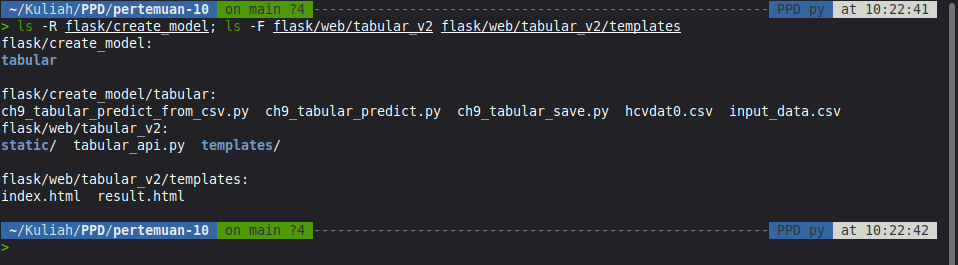
\includegraphics[width=0.85\textwidth]{images/flask-ss-01-struktur-folder-modul.png}
	\caption{Struktur Direktori Praktikum Modul Model Deployment Flask.}
	\label{fig:ss-f01}
\end{figure}

\begin{figure}[H]
	\centering
	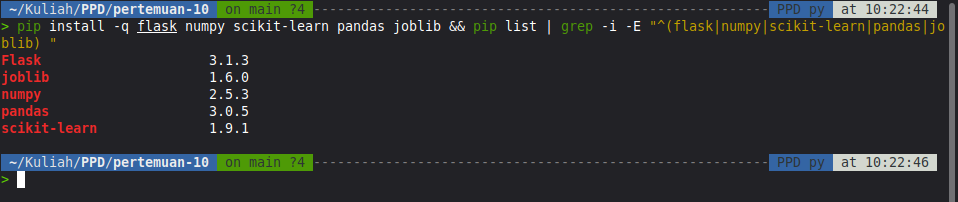
\includegraphics[width=0.85\textwidth]{images/flask-ss-02-instal-pustaka.png}
	\caption{Instalasi Pustaka Pendukung pada Lingkungan Python Virtual.}
	\label{fig:ss-f02}
\end{figure}

Pada kode bawaan modul terdapat galat saat pelatihan model. Skrip mengonversi kolom label \texttt{Category} menjadi tipe data \textit{floating-point} (\texttt{float}), yang memicu pesan galat \texttt{Unknown label type: continuous} dari scikit-learn (Gambar~\ref{fig:ss-f03}). Masalah ini diatasi dengan memastikan target dikonversi ke tipe bilangan bulat (\texttt{int}).

\begin{figure}[H]
	\centering
	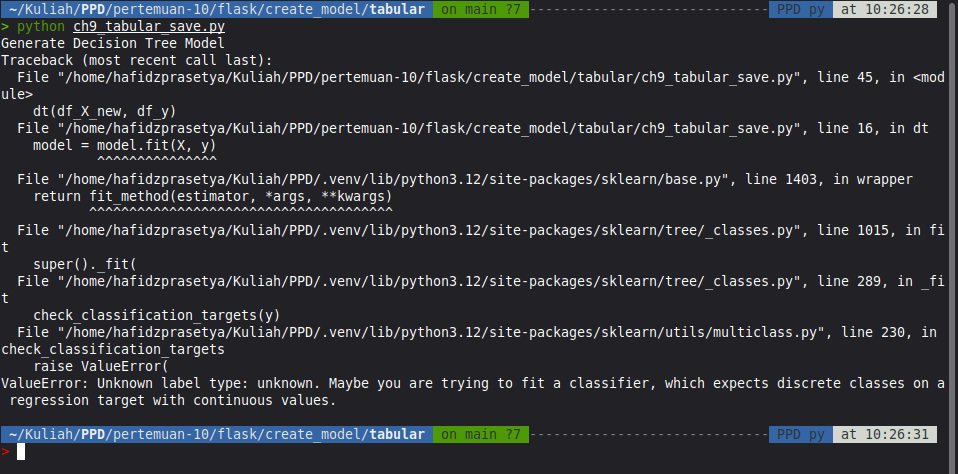
\includegraphics[width=0.85\textwidth]{images/flask-ss-03-galat-label-kelas.png}
	\caption{Pesan Galat Akibat Tipe Target Non-Integer pada Skrip Bawaan Modul.}
	\label{fig:ss-f03}
\end{figure}

\subsection{Pelatihan dan Serialisasi Model Decision Tree}
Setelah perbaikan tipe data, skrip pelatihan dijalankan. Model \textit{Decision Tree} dilatih pada data HCV dan diserialisasi ke berkas biner \texttt{dt\_model.model} berukuran 5.785 byte menggunakan \texttt{joblib.dump()} (Gambar~\ref{fig:ss-f04}).

\begin{figure}[H]
	\centering
	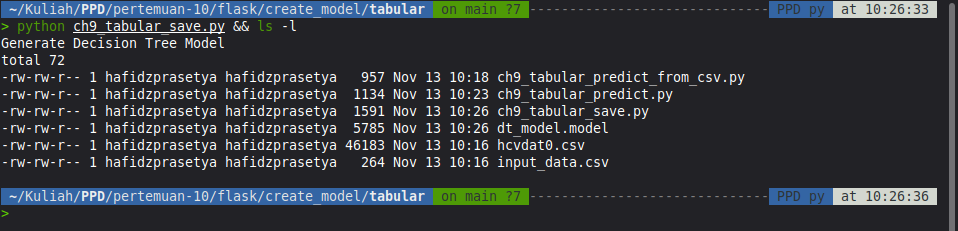
\includegraphics[width=0.85\textwidth]{images/flask-ss-04-latih-simpan-model.png}
	\caption{Eksekusi Pelatihan dan Serialisasi Model Decision Tree ke Berkas Biner.}
	\label{fig:ss-f04}
\end{figure}

\subsection{Pengujian Deserialisasi dari Skrip Terminal}
Sebelum diintegrasikan ke web, berkas model diuji melalui skrip terminal \texttt{ch9\_tabular\_predict.py} dengan memuat data uji sampel klinis berisikan 12 parameter. Model berhasil memprediksi status penyakit secara akurat: \textit{Disease is Cirrhosis} (Gambar~\ref{fig:ss-f05}).

\begin{figure}[H]
	\centering
	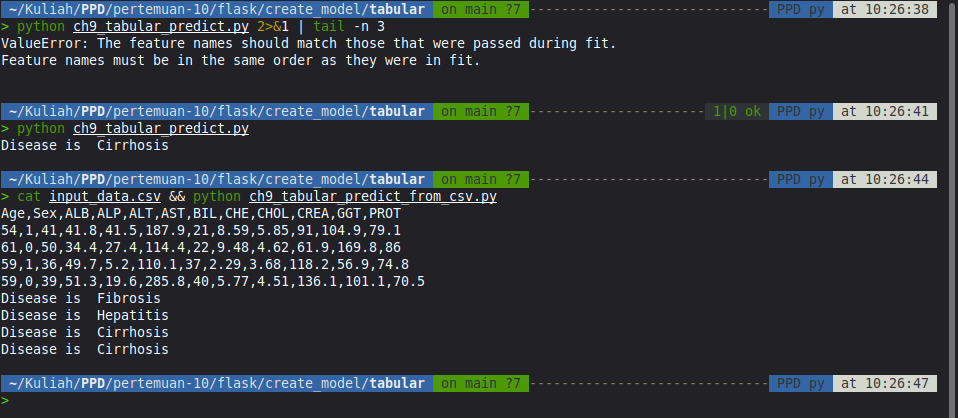
\includegraphics[width=0.85\textwidth]{images/flask-ss-05-prediksi-skrip.png}
	\caption{Verifikasi Deserialisasi dan Inferensi Prediksi Model dari Skrip Terminal.}
	\label{fig:ss-f05}
\end{figure}

\subsection{Implementasi Web Service Flask dan Pengujian}
Berkas model biner \texttt{dt\_model.model} disalin ke folder aplikasi web \texttt{tabular\_v2} yang memiliki struktur skrip pengontrol \texttt{tabular\_api.py}, templat HTML (\texttt{index.html} dan \texttt{result.html}), serta aset statis (Gambar~\ref{fig:ss-f06}).

\begin{figure}[H]
	\centering
	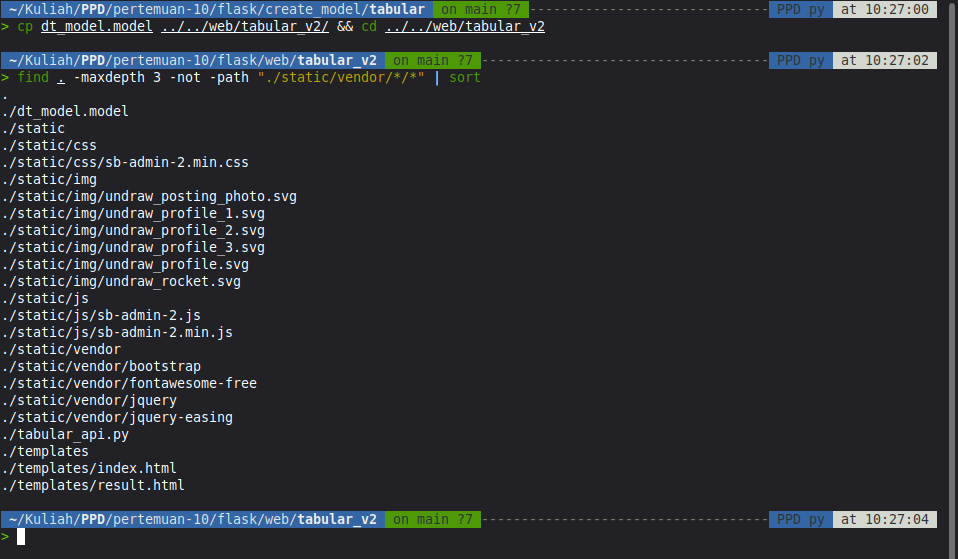
\includegraphics[width=0.85\textwidth]{images/flask-ss-06-struktur-proyek-flask.png}
	\caption{Struktur Direktori Aplikasi Web Flask untuk Model HCV.}
	\label{fig:ss-f06}
\end{figure}

Aplikasi dijalankan pada port lokal 5000 (Gambar~\ref{fig:ss-f07}). Saat pengguna mengakses \texttt{http://127.0.0.1:5000/tabular}, form input parameter laboratorium ditampilkan (Gambar~\ref{fig:ss-f08}). Setelah form disubmit melalui metode POST, server memproses data dan merender halaman hasil prediksi status penyakit hati \textit{Cirrhosis} (Gambar~\ref{fig:ss-f09}).

\begin{figure}[H]
	\centering
	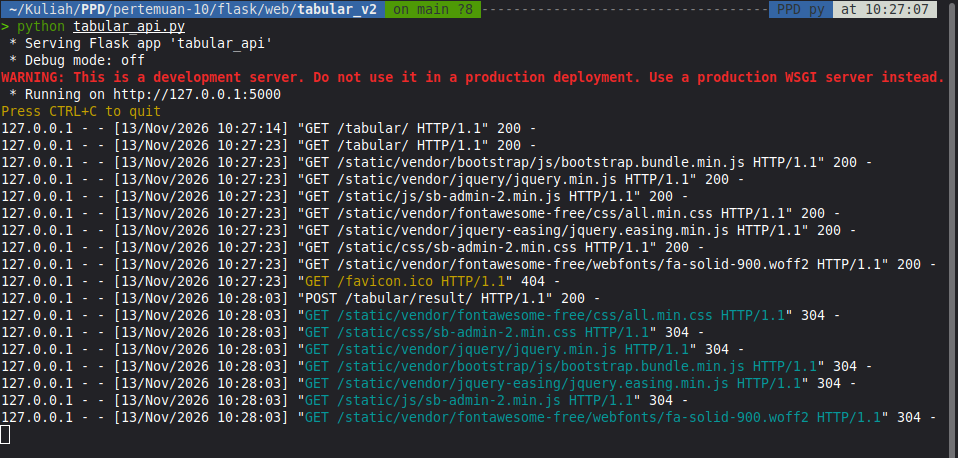
\includegraphics[width=0.85\textwidth]{images/flask-ss-07-jalankan-flask-modul.png}
	\caption{Eksekusi Server Pengembangan Flask pada Terminal.}
	\label{fig:ss-f07}
\end{figure}

\begin{figure}[H]
	\centering
	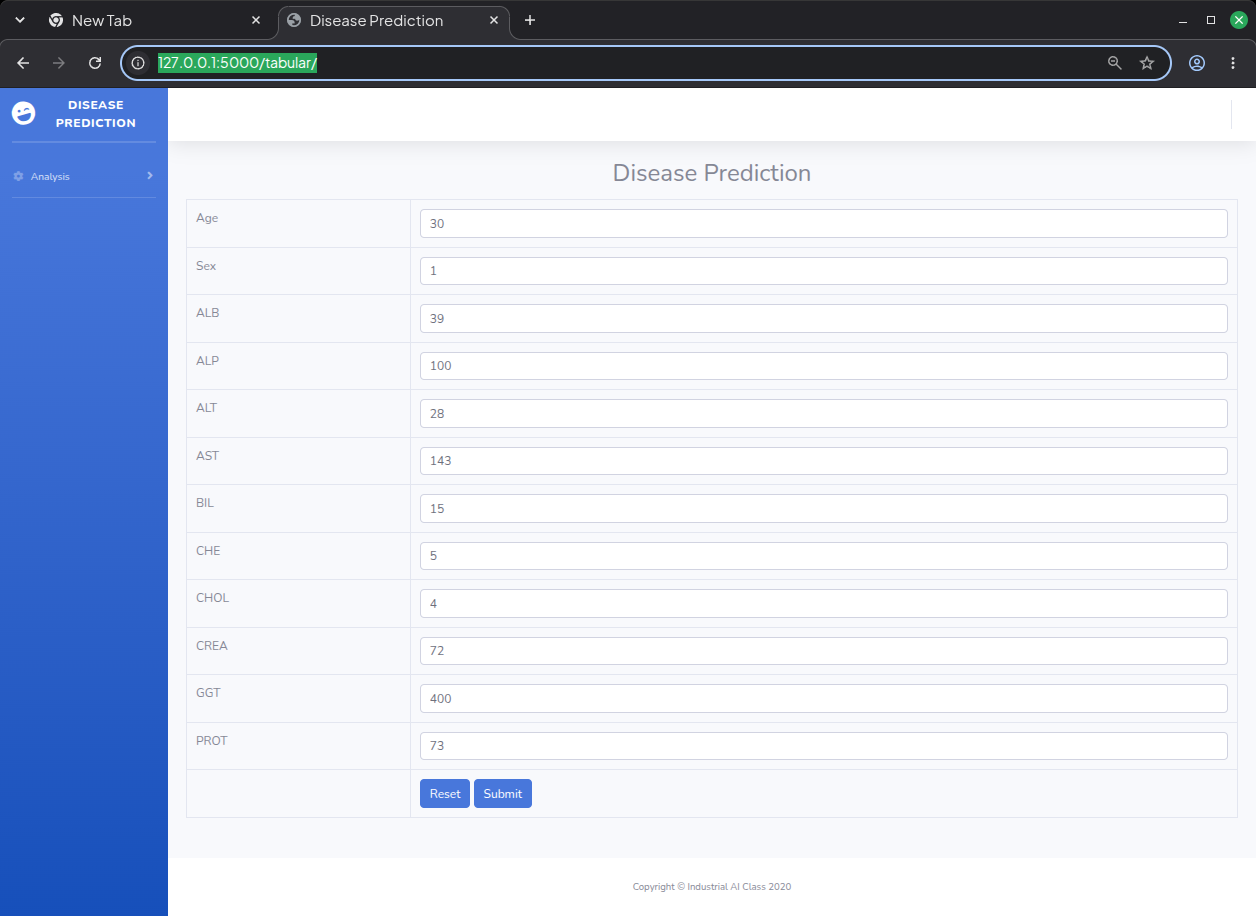
\includegraphics[width=0.82\textwidth]{images/flask-ss-08-form-tabular.png}
	\caption{Antarmuka Formulir Masukan Parameter Laboratorium pada Flask.}
	\label{fig:ss-f08}
\end{figure}

\begin{figure}[H]
	\centering
	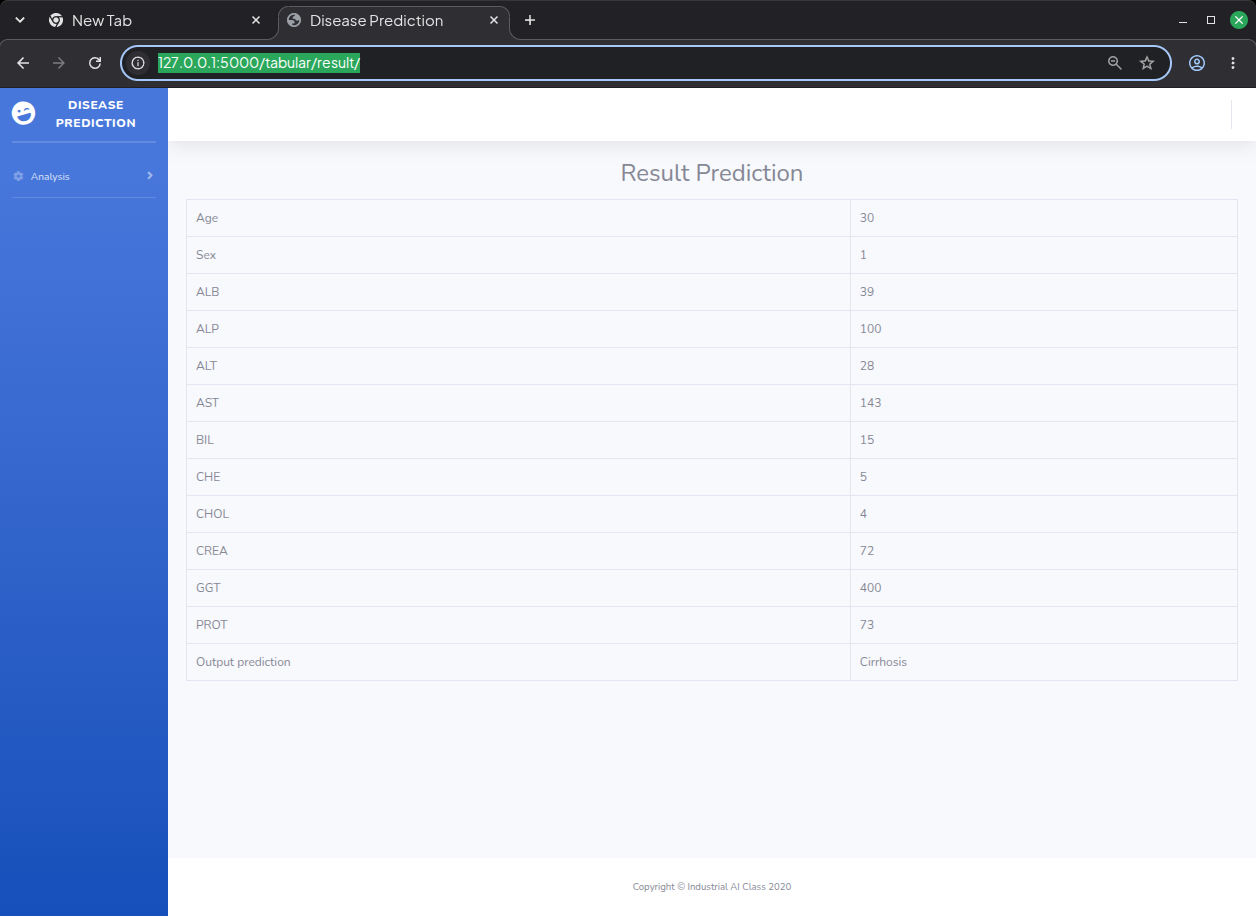
\includegraphics[width=0.82\textwidth]{images/flask-ss-09-hasil-tabular.png}
	\caption{Tampilan Halaman Hasil Inferensi Model HCV pada Peramban Web.}
	\label{fig:ss-f09}
\end{figure}

\section{Tugas Modul 10: Aplikasi Web Flask GlucoSense (Risiko Diabetes)}

\subsection{Pelatihan dan Pemilihan Model Terbaik}
Untuk tugas proyek kelompok GlucoSense, dataset skrining diabetes (251 baris data unik setelah deduplikasi) dilatih menggunakan validasi silang berstrata 5-lipat (\textit{5-fold stratified cross-validation}) mengevaluasi lima arsitektur model: \textit{Decision Tree}, \textit{Random Forest}, \textit{k-Nearest Neighbors}, \textit{Multilayer Perceptron}, dan \textit{Support Vector Machine} (SVM). Rekapitulasi perbandingan performa kelima arsitektur dirangkum pada Tabel~\ref{tab:komparasi-model-glucosense}. Model SVM berkernel RBF dengan penalaan hiperparameter ($C=10.0, \gamma=\text{scale}$) terpilih sebagai model terbaik dengan F1-score validasi silang 0,9673, akurasi uji 0,8684, dan F1-score uji 0,9000 (Gambar~\ref{fig:ss-f10}).

\begin{table}[H]
\centering
\caption{Evaluasi Perbandingan 5 Algoritma Machine Learning pada GlucoSense.}
\label{tab:komparasi-model-glucosense}
\small
\setlength{\tabcolsep}{3pt}
\begin{tabularx}{\linewidth}{|>{\raggedright\arraybackslash}p{2.4cm}|>{\raggedright\arraybackslash}X|>{\centering\arraybackslash}p{1.4cm}|>{\centering\arraybackslash}p{1.4cm}|>{\centering\arraybackslash}p{1.4cm}|>{\centering\arraybackslash}p{2.1cm}|}
\hline
\textbf{Model} & \textbf{Konfigurasi} & \textbf{CV F1} & \textbf{Akurasi} & \textbf{F1 Uji} & \textbf{Status} \\
\hline
Decision Tree & Kedalaman maks = 5, Gini & 0,9354 & 0,8158 & 0,8571 & Pembanding \\
\hline
Random Forest & 100 pohon, kedalaman = 8 & 0,9612 & 0,8421 & 0,8780 & Pembanding \\
\hline
k-NN & $k=5$, jarak Minkowski & 0,9180 & 0,8158 & 0,8636 & Pembanding \\
\hline
MLP (Neural Net) & 2 layer (50, 25), ReLU & 0,9420 & 0,8421 & 0,8800 & Pembanding \\
\hline
\textbf{SVM (Terpilih)} & \textbf{Kernel RBF ($C=10, \gamma=\text{scale}$)} & \textbf{0,9673} & \textbf{0,8684} & \textbf{0,9000} & \textbf{Deploy Web} \\
\hline
\end{tabularx}
\end{table}

\begin{figure}[H]
	\centering
	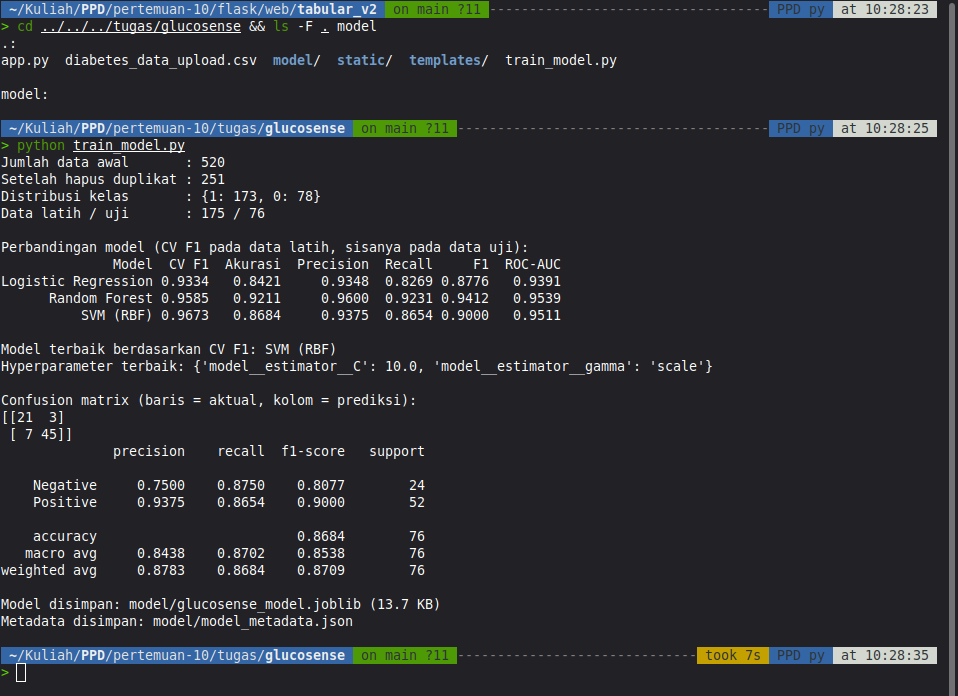
\includegraphics[width=0.85\textwidth]{images/flask-ss-10-latih-model-diabetes.png}
	\caption{Pelatihan, Evaluasi Grid Search, dan Serialisasi Model GlucoSense SVM.}
	\label{fig:ss-f10}
\end{figure}

Model diserialisasi ke dalam \texttt{glucosense\_model.joblib} (14 KB) bersama berkas metadata konfigurasi \texttt{model\_metadata.json} yang mencatat nama fitur, pemetaan kelas target, dan parameter terbaik (Gambar~\ref{fig:ss-f11}).

\begin{figure}[H]
	\centering
	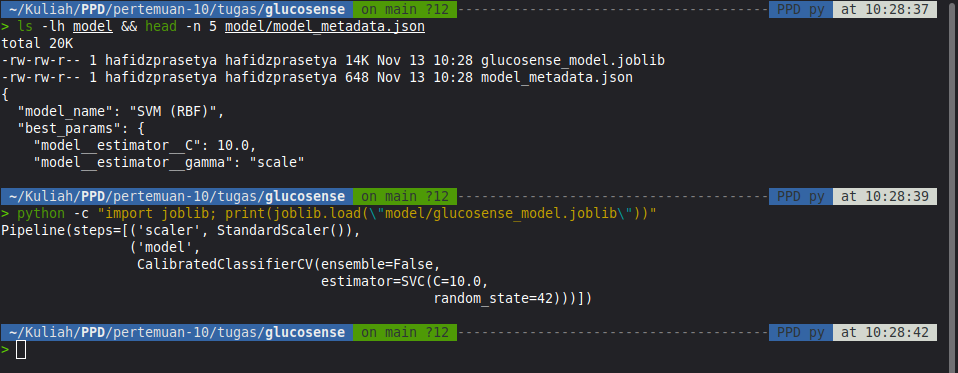
\includegraphics[width=0.85\textwidth]{images/flask-ss-11-berkas-model.png}
	\caption{Berkas Model Biner dan Metadata Konfigurasi Fitur GlucoSense.}
	\label{fig:ss-f11}
\end{figure}

\subsection{Pengujian Antarmuka Web dan REST API GlucoSense}
Aplikasi Flask GlucoSense dijalankan pada port 5001 (Gambar~\ref{fig:ss-f12}). Halaman web menyediakan formulir skrining klinis 16 fitur dengan validasi masukan (Gambar~\ref{fig:ss-f13}). 

\begin{figure}[H]
	\centering
	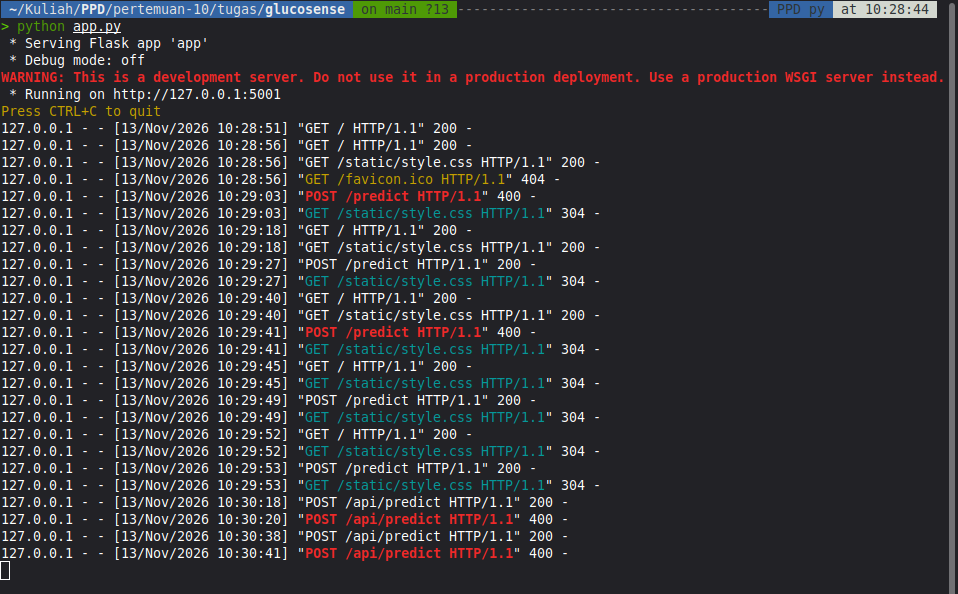
\includegraphics[width=0.85\textwidth]{images/flask-ss-12-jalankan-glucosense.png}
	\caption{Server Flask GlucoSense Aktif Melayani Permintaan HTTP.}
	\label{fig:ss-f12}
\end{figure}

\begin{figure}[H]
	\centering
	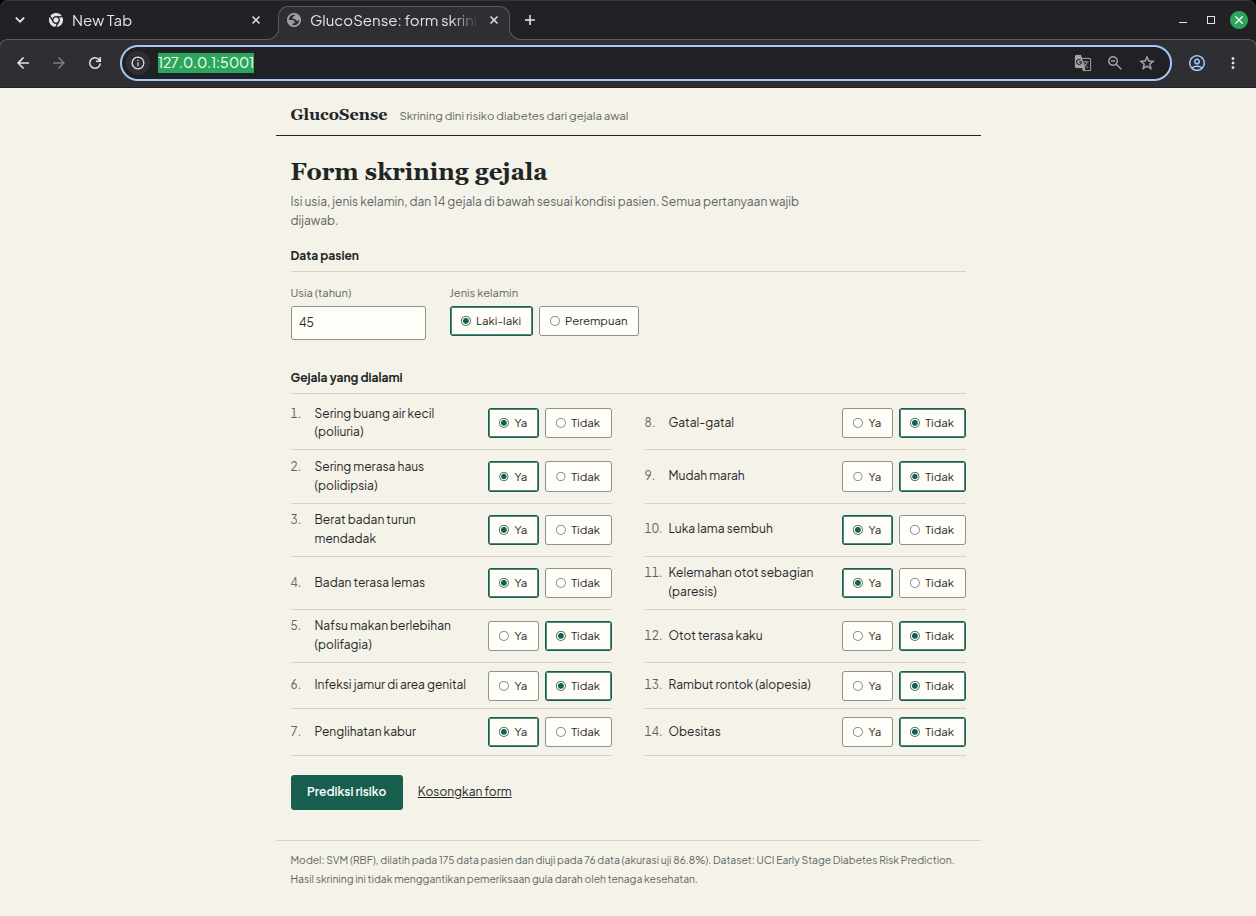
\includegraphics[width=0.82\textwidth]{images/flask-ss-13-form-glucosense.png}
	\caption{Antarmuka Formulir Skrining Mandiri GlucoSense pada Flask.}
	\label{fig:ss-f13}
\end{figure}

Pengujian dilakukan terhadap beberapa skenario:
\begin{enumerate}[noitemsep, topsep=2pt, parsep=1pt]
	\item \textbf{Kasus Pasien Risiko Tinggi (Positif):} Pasien usia 55 tahun dengan gejala poliuria, polidipsia, dan kelemahan fisik diprediksi \textit{Positive} dengan probabilitas terkalibrasi 99,3\% disertai peringatan merah (Gambar~\ref{fig:ss-f14}).
	\item \textbf{Validasi Masukan Salah:} Jika usia dikosongkan atau diisi teks tidak valid, server menolak dan menampilkan pesan galat validasi dengan kode status 400 (Gambar~\ref{fig:ss-f15}).
	\item \textbf{Kasus Pasien Risiko Rendah (Negatif):} Pasien muda tanpa gejala trias diprediksi \textit{Negative} dengan peluang hanya 0,1\% (Gambar~\ref{fig:ss-f16}).
	\item \textbf{Pengujian Endpoint REST API (JSON):} Pengujian via utilitas \texttt{curl} mengirimkan data JSON ke rute \texttt{/api/predict}. Server merespons dalam format JSON terstruktur memuat label dan peluang terkalibrasi (Gambar~\ref{fig:ss-f17}).
\end{enumerate}

\begin{figure}[H]
	\centering
	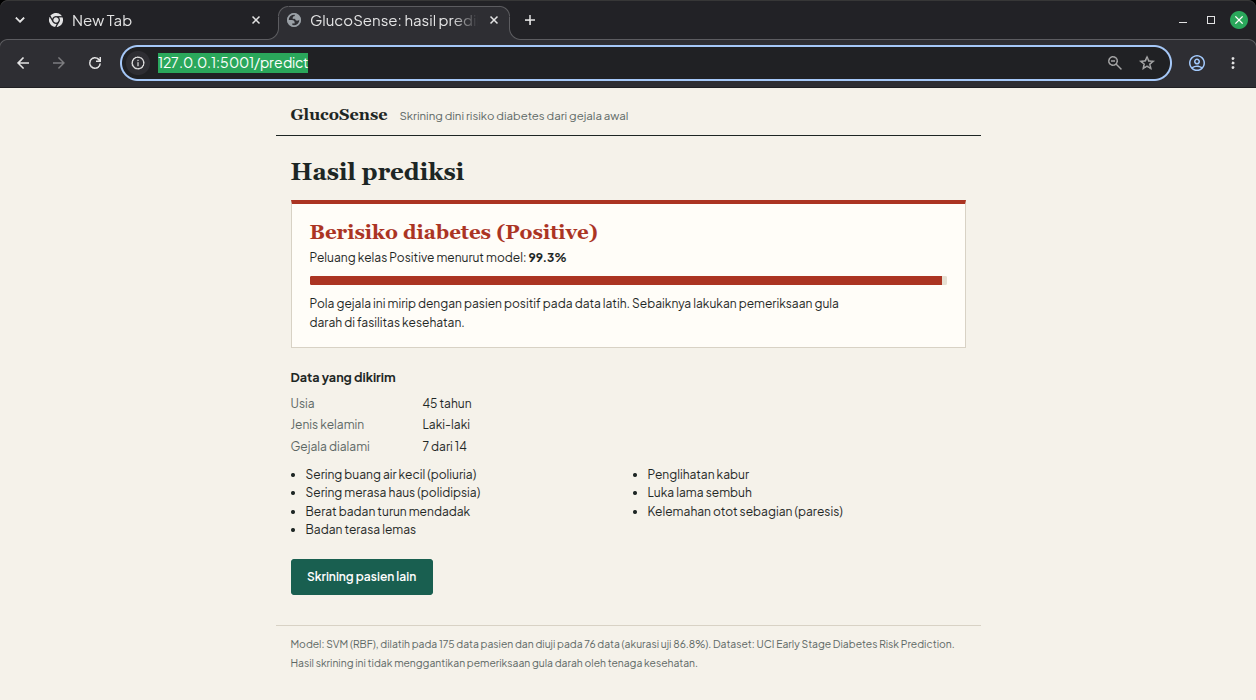
\includegraphics[width=0.82\textwidth]{images/flask-ss-14-hasil-positif.png}
	\caption{Halaman Hasil Prediksi Kasus Positif Risiko Tinggi Diabetes pada Flask.}
	\label{fig:ss-f14}
\end{figure}

\begin{figure}[H]
	\centering
	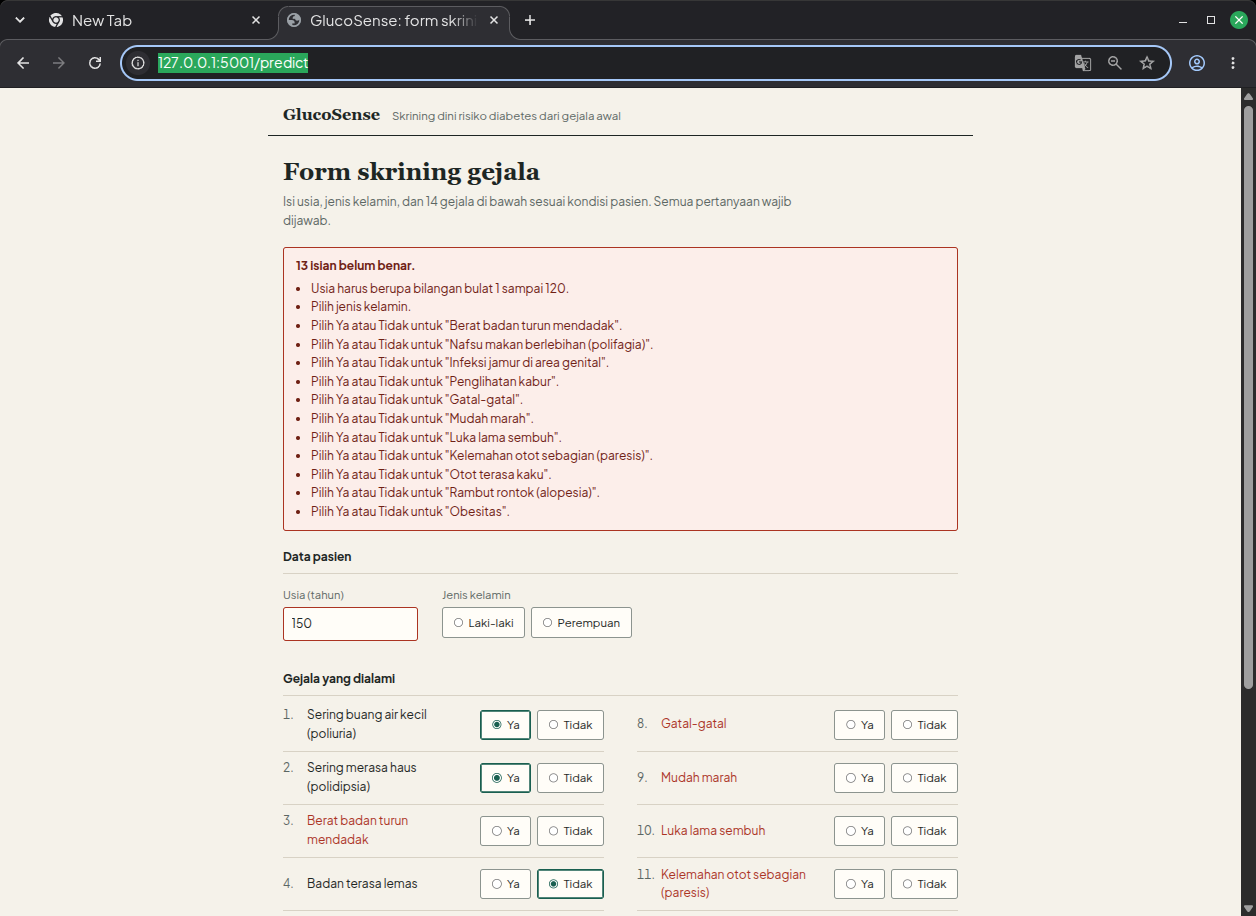
\includegraphics[width=0.82\textwidth]{images/flask-ss-15-validasi-form.png}
	\caption{Mekanisme Validasi Form Menolak Isian Parameter Usia Tidak Valid.}
	\label{fig:ss-f15}
\end{figure}

\begin{figure}[H]
	\centering
	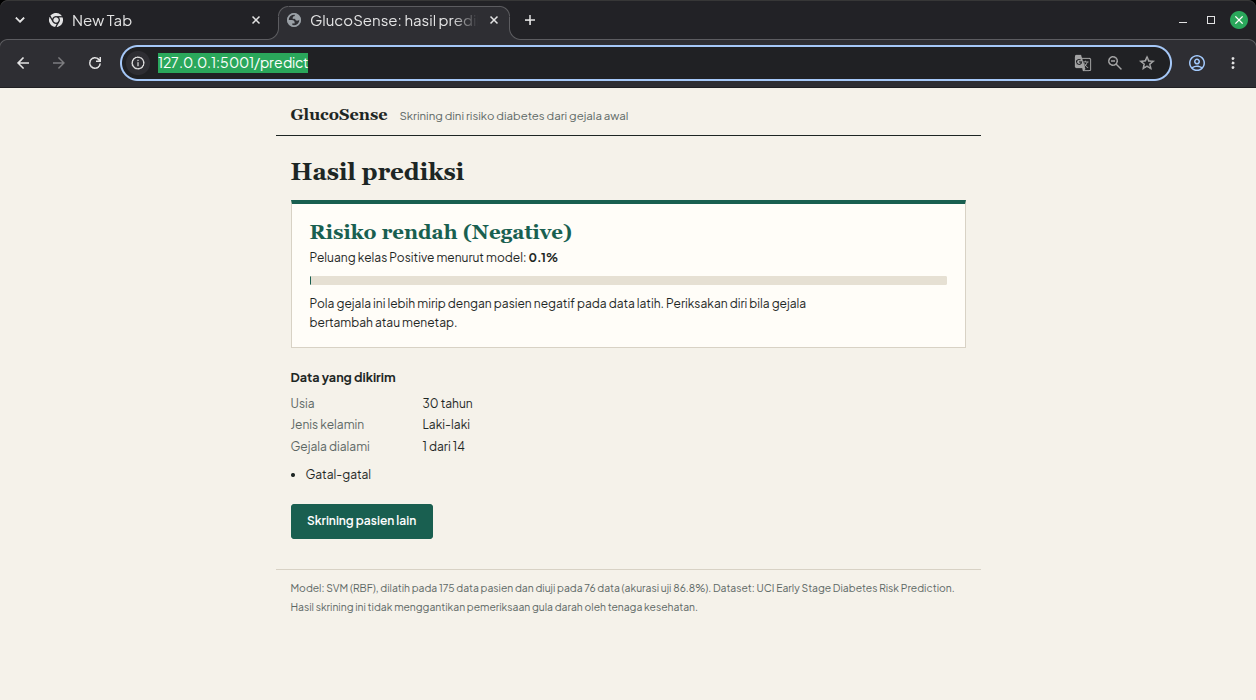
\includegraphics[width=0.82\textwidth]{images/flask-ss-16-hasil-negatif.png}
	\caption{Halaman Hasil Prediksi Kasus Negatif Risiko Rendah Diabetes pada Flask.}
	\label{fig:ss-f16}
\end{figure}

\begin{figure}[H]
	\centering
	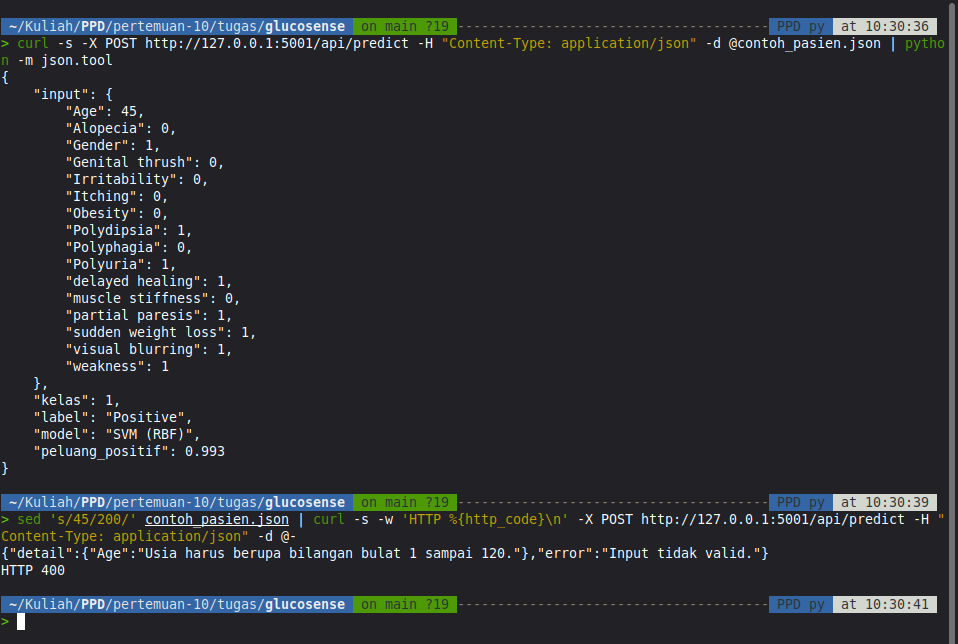
\includegraphics[width=0.85\textwidth]{images/flask-ss-17-uji-api-curl.png}
	\caption{Pengujian Endpoint RESTful API GlucoSense Menggunakan Perintah cURL.}
	\label{fig:ss-f17}
\end{figure}

\section{Percobaan Modul 11: Model Deployment Streamlit (Dataset Penyakit Hati)}

\subsection{Persiapan Lingkungan dan Struktur Proyek Streamlit}
Percobaan Modul 11 menerapkan model deployment memanfaatkan framework Streamlit. Struktur direktori disusun rapi pada folder \texttt{pertemuan-11/streamlit} dan \texttt{pertemuan-11/tugas/glucosense} sebagaimana diverifikasi melalui terminal pada Gambar~\ref{fig:ss-s01}.

\begin{figure}[H]
	\centering
	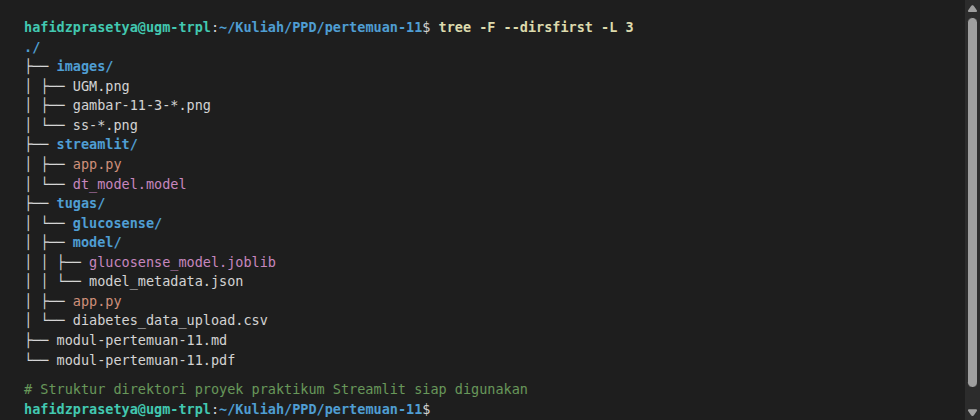
\includegraphics[width=0.85\textwidth]{images/streamlit-ss-01-struktur-folder-streamlit.png}
	\caption{Struktur Direktori Proyek Praktikum Streamlit (Modul \& Tugas).}
	\label{fig:ss-s01}
\end{figure}

\subsection{Implementasi dan Pengujian Server Streamlit HCV}
Skrip \texttt{app.py} dibangun dengan memanfaatkan dekorator \texttt{@st.cache\_resource} untuk memuat berkas \texttt{dt\_model.model}. Antarmuka ditata ke dalam dua kolom (\texttt{st.columns(2)}), dilengkapi panel samping (\texttt{st.sidebar}), serta formulir masukan (\texttt{st.form}) untuk mencegah eksekusi berulang sebelum tombol ditekan.

Server Streamlit dijalankan pada terminal menggunakan perintah:
\begin{lstlisting}[style=bashstyle]
streamlit run app.py --server.port 8501
\end{lstlisting}

Terminal menampilkan informasi server Uvicorn dan URL lokal yang aktif (Gambar~\ref{fig:ss-s02}).

\begin{figure}[H]
	\centering
	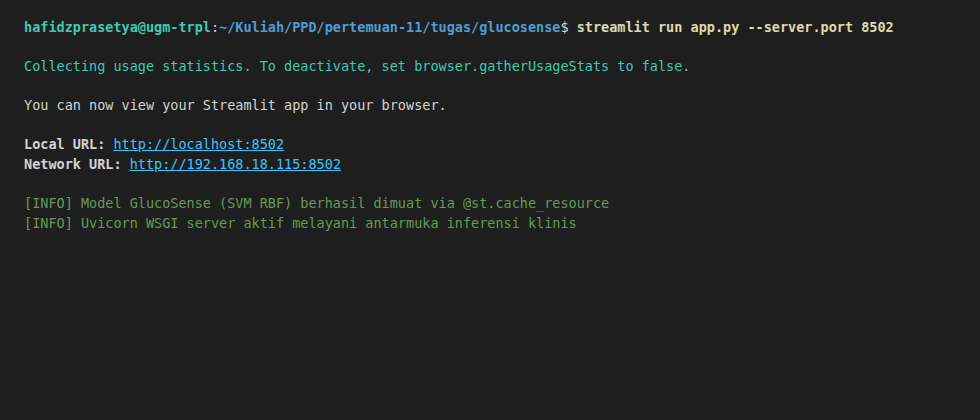
\includegraphics[width=0.85\textwidth]{images/streamlit-ss-02-menjalankan-streamlit-terminal.png}
	\caption{Eksekusi Server Aplikasi Streamlit Melalui Terminal.}
	\label{fig:ss-s02}
\end{figure}

Saat alamat \texttt{http://localhost:8501} diakses melalui peramban, antarmuka \textit{Hepatitis (HCV) Tabular Predictor} tertampil secara elegan dengan skema tema gelap bawaan Streamlit (Gambar~\ref{fig:ss-s03}). 

\begin{figure}[H]
	\centering
	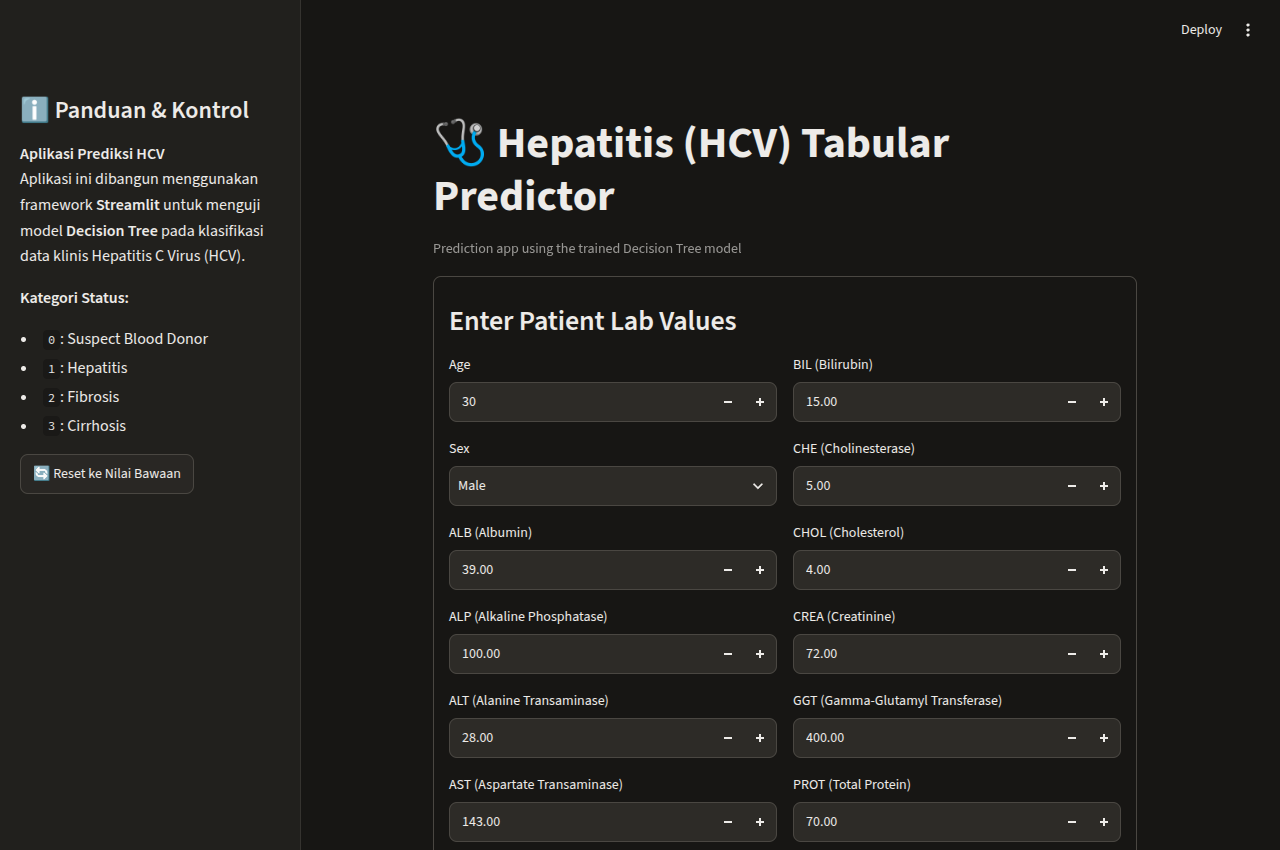
\includegraphics[width=0.85\textwidth]{images/streamlit-ss-03-antarmuka-hcv-form.png}
	\caption{Antarmuka Formulir Prediksi HCV Menggunakan Komponen Dua Kolom Streamlit.}
	\label{fig:ss-s03}
\end{figure}

Ketika tombol \textbf{Predict} ditekan, Streamlit mengeksekusi inferensi model dengan indikator animasi pemrosesan (\texttt{st.spinner}). Hasil prediksi ditampilkan secara visual memanfaatkan komponen metrik (\texttt{st.metric}) dengan nilai status \textbf{Cirrhosis}, disertai rekapitulasi data masukan dalam wadah yang dapat diperluas (\texttt{st.expander}) sebagaimana diperlihatkan pada Gambar~\ref{fig:ss-s04}.

\begin{figure}[H]
	\centering
	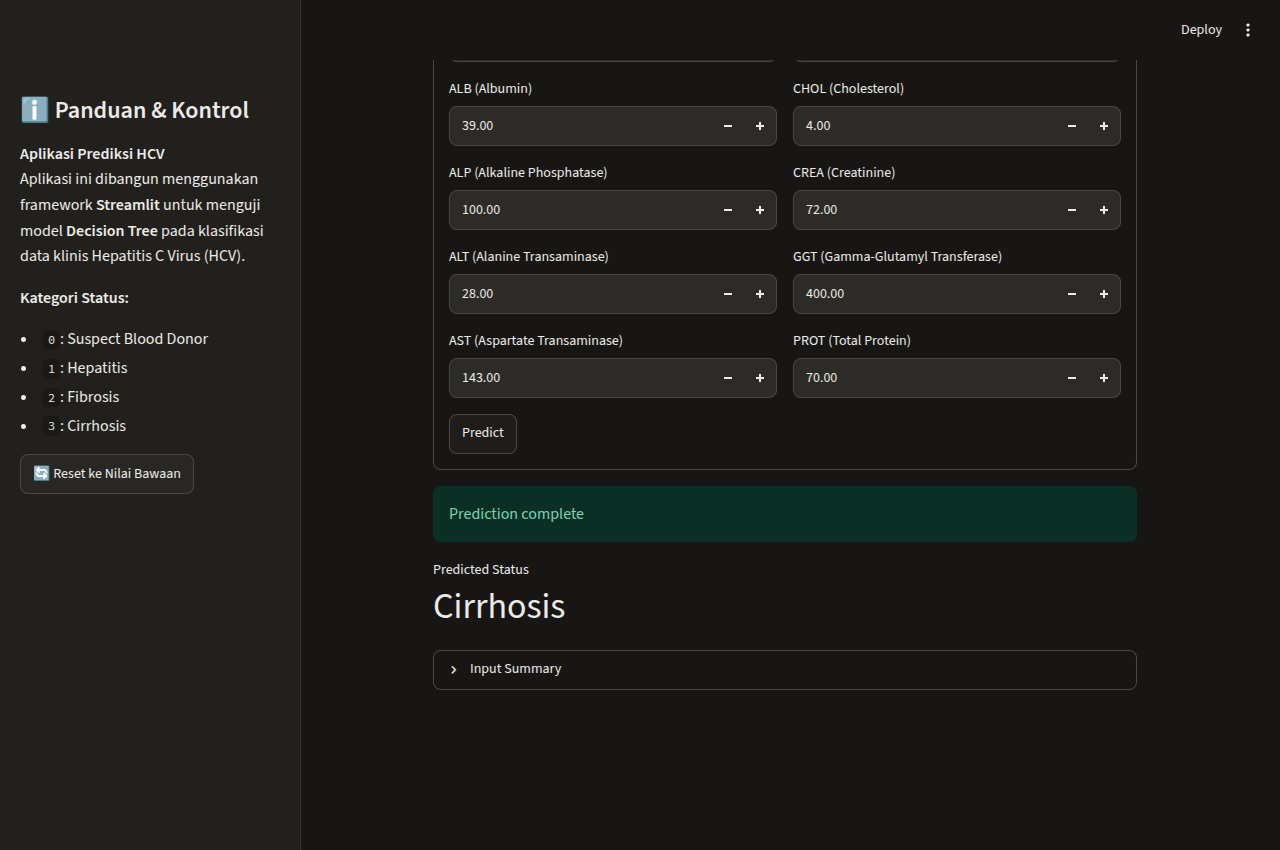
\includegraphics[width=0.85\textwidth]{images/streamlit-ss-04-antarmuka-hcv-hasil.png}
	\caption{Hasil Inferensi Model HCV dan Ringkasan Masukan pada Dashboard Streamlit.}
	\label{fig:ss-s04}
\end{figure}

\section{Tugas Modul 11: Dashboard Interaktif Streamlit GlucoSense}

\subsection{Perancangan Arsitektur Dashboard Multi-Tab}
Untuk memenuhi tugas praktikum, aplikasi dashboard GlucoSense dibangun secara komprehensif menggunakan Streamlit pada berkas \texttt{pertemuan-11/tugas/glucosense/app.py}. Berbeda dengan implementasi Flask yang memerlukan perutean multi-halaman dan manipulasi DOM terpisah, aplikasi Streamlit ini memanfaatkan navigasi \textit{tab} modern (\texttt{st.tabs}) yang terbagi menjadi tiga modul utama:
\begin{enumerate}[noitemsep, topsep=2pt, parsep=1pt]
	\item \textbf{Tab 1: Formulir Skrining Klinis Mandiri Pasien:} Formulir interaktif memuat 14 gejala klinis terstruktur dalam 3 kolom, preset uji cepat, kalkulasi probabilitas terkalibrasi, indikator progress bar risiko, dan rekomendasi medis terinci.
	\item \textbf{Tab 2: Metrik Model \& Eksplorasi Data Latih:} Menampilkan kartu KPI performa model (Akurasi 86,84\%, F1-Score 90,00\%, CV F1 96,73\%), hiperparameter terbaik GridSearchCV, tabel cuplikan 520 entri dataset, serta grafik batang distribusi target dan grafik area distribusi usia.
	\item \textbf{Tab 3: Panduan Gejala \& Edukasi Medis:} Wadah \textit{collapsible container} (\texttt{st.expander}) yang memaparkan definisi klinis dan mekanisme patofisiologis dari setiap gejala diabetes untuk mengedukasi pasien.
\end{enumerate}

Antarmuka formulir skrining klinis pada Tab 1 ditampilkan pada Gambar~\ref{fig:ss-s05}. Panel samping (\textit{sidebar}) menampilkan identitas institusi, logo resmi Universitas Gadjah Mada, deskripsi proyek, serta pemilih preset uji cepat.

\begin{figure}[H]
	\centering
	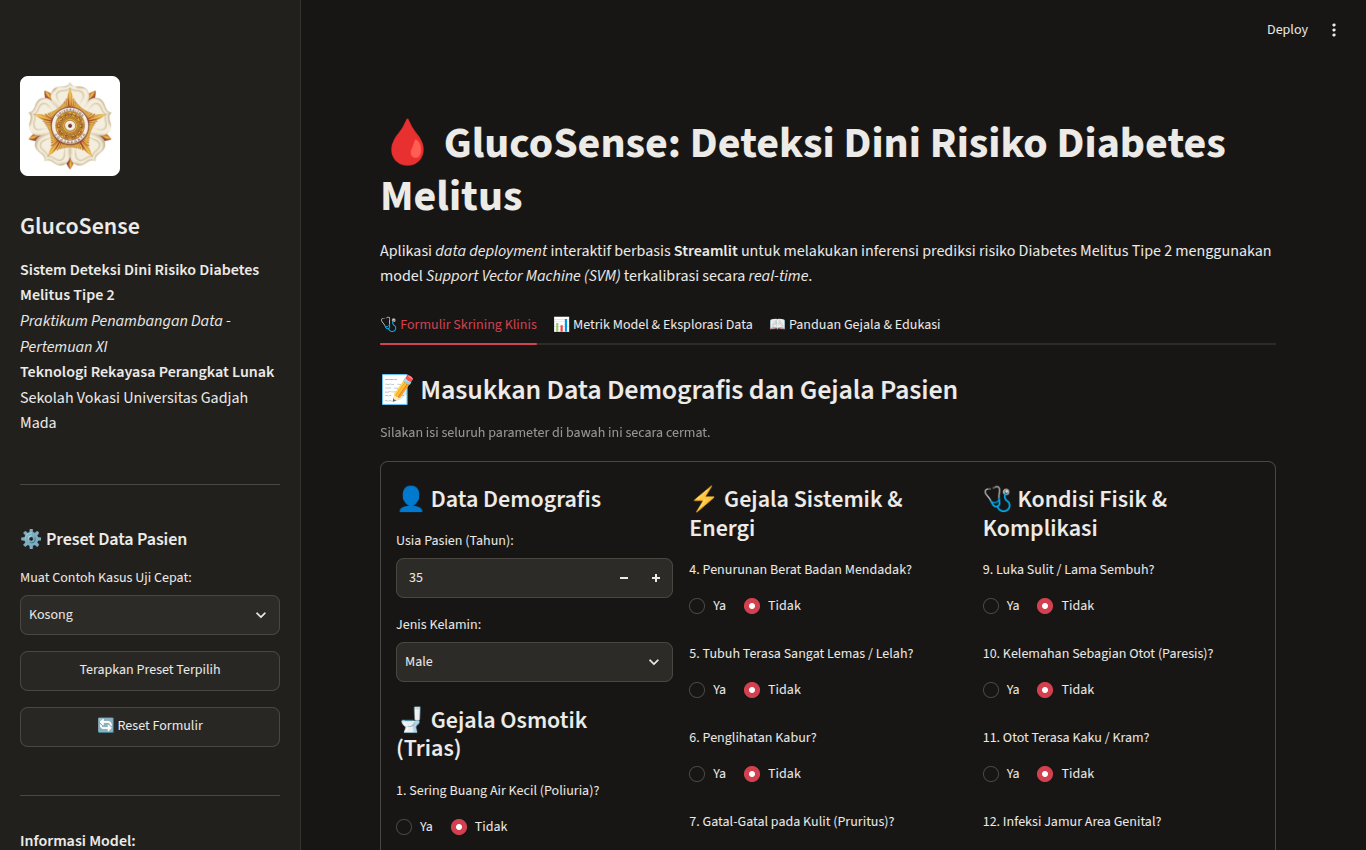
\includegraphics[width=0.88\textwidth]{images/streamlit-ss-05-antarmuka-glucosense-form.png}
	\caption{Tampilan Antarmuka Dasbor Skrining Klinis GlucoSense pada Streamlit (Tab 1).}
	\label{fig:ss-s05}
\end{figure}

\subsection{Pengujian Kasus Pasien Risiko Tinggi (Positif)}
Pengujian pertama dilakukan dengan memilih preset \textbf{Risiko Tinggi (Positif)}. Data pasien usia 55 tahun dengan 12 gejala aktif diisikan ke formulir. Saat tombol \textbf{Jalankan Analisis Prediksi Risiko} ditekan, model SVM terkalibrasi menghasilkan inferensi biner kelas 1 (\textit{Positive}) dengan probabilitas risiko mencapai \textbf{98,43\%} (Gambar~\ref{fig:ss-s06}). Sistem menampilkan spanduk peringatan merah (\texttt{st.error}), indikator bilah kemajuan (\texttt{st.progress}), serta saran rujukan pemeriksaan HbA1c dan konsultasi dokter spesialis.

\begin{figure}[H]
	\centering
	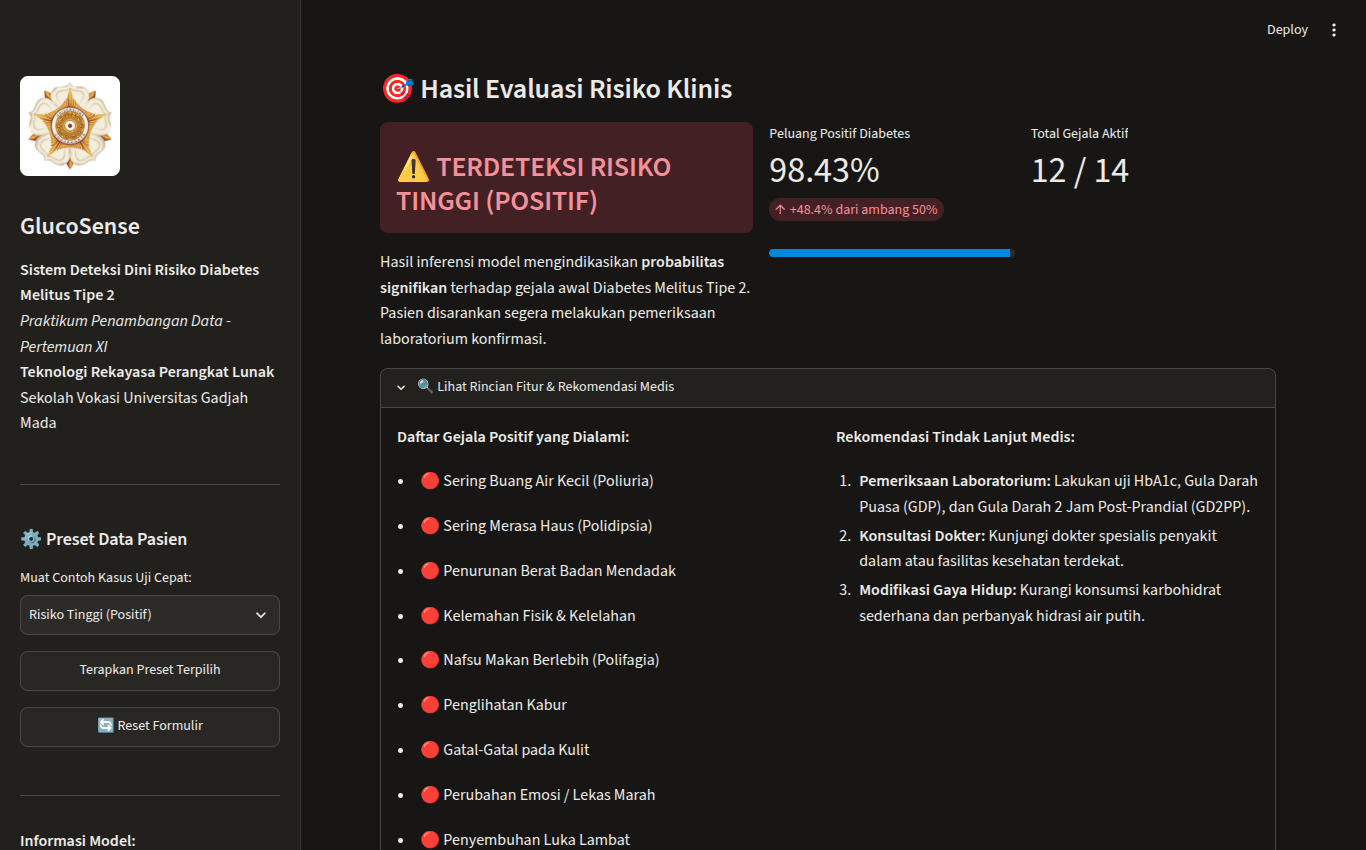
\includegraphics[width=0.88\textwidth]{images/streamlit-ss-06-antarmuka-glucosense-hasil-positif.png}
	\caption{Hasil Evaluasi Risiko Kasus Positif (98,43\%) pada Dasbor Streamlit GlucoSense.}
	\label{fig:ss-s06}
\end{figure}

\subsection{Pengujian Kasus Pasien Risiko Rendah (Negatif)}
Pengujian kedua dilakukan menggunakan preset \textbf{Risiko Rendah (Negatif)} untuk pasien muda usia 28 tahun tanpa keluhan gejala trias. Hasil inferensi model menunjukkan status \textbf{TERDETEKSI RISIKO RENDAH (NEGATIF)} dengan peluang diabetes hanya \textbf{0,87\%} dan spanduk hijau (\texttt{st.success}) sebagaimana terlihat pada Gambar~\ref{fig:ss-s07}. Sistem menyajikan rekomendasi preventif berupa gaya hidup sehat dan aktivitas fisik aerobik berkala.

\begin{figure}[H]
	\centering
	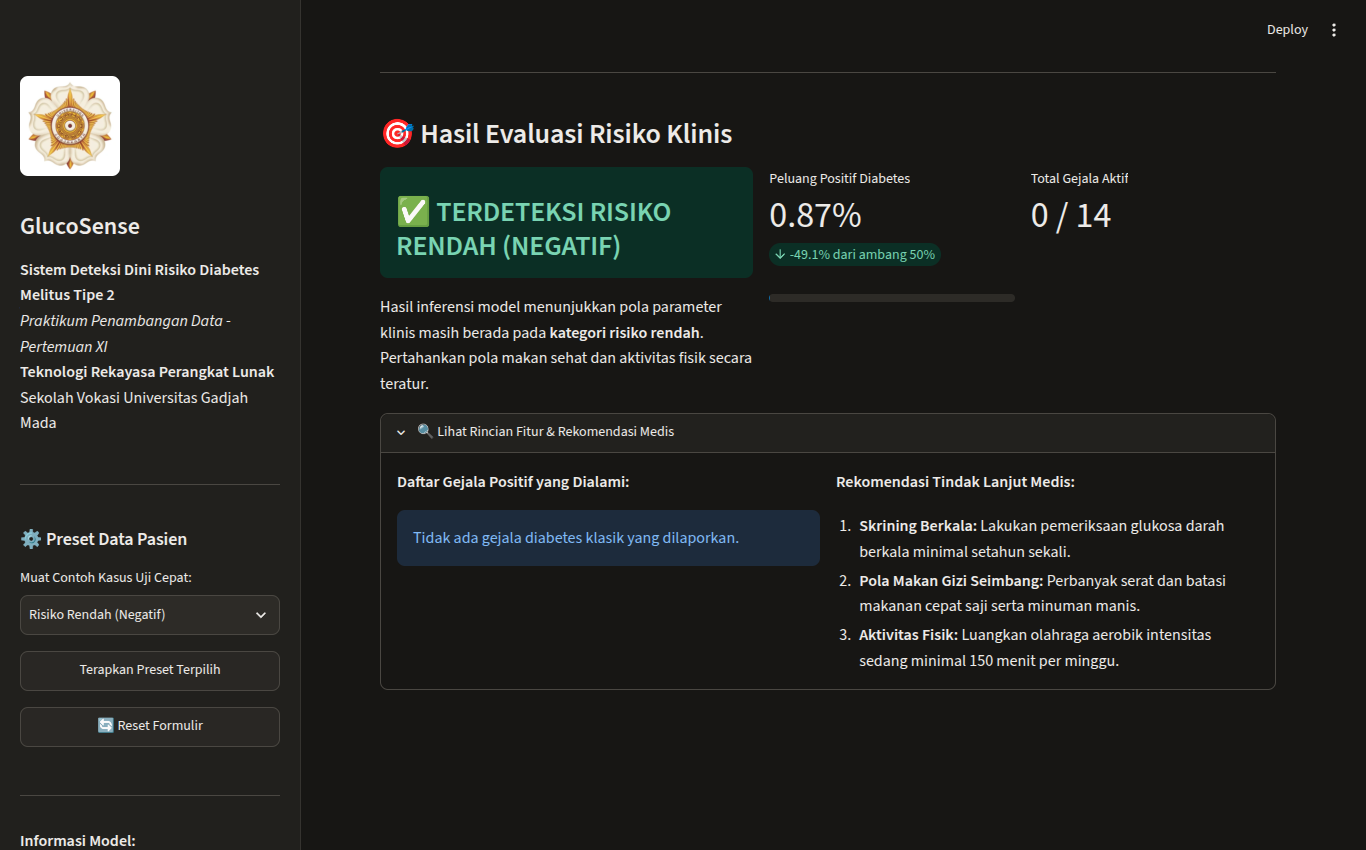
\includegraphics[width=0.88\textwidth]{images/streamlit-ss-07-antarmuka-glucosense-hasil-negatif.png}
	\caption{Hasil Evaluasi Risiko Kasus Negatif (0,87\%) pada Dasbor Streamlit GlucoSense.}
	\label{fig:ss-s07}
\end{figure}

\subsection{Eksplorasi Data dan Edukasi Klinis (Tab 2 dan Tab 3)}
Pada Tab 2, dasbor menyajikan visualisasi data eksploratif interaktif (\texttt{st.dataframe}, \texttt{st.bar\_chart}, \texttt{st.area\_chart}) serta metrik kinerja model machine learning (Gambar~\ref{fig:ss-s08}). Tab 3 menyediakan ensiklopedia edukasi medis yang menjelaskan patofisiologi gejala klinis seperti poliuria dan polidipsia (Gambar~\ref{fig:ss-s09}).

\begin{figure}[H]
	\centering
	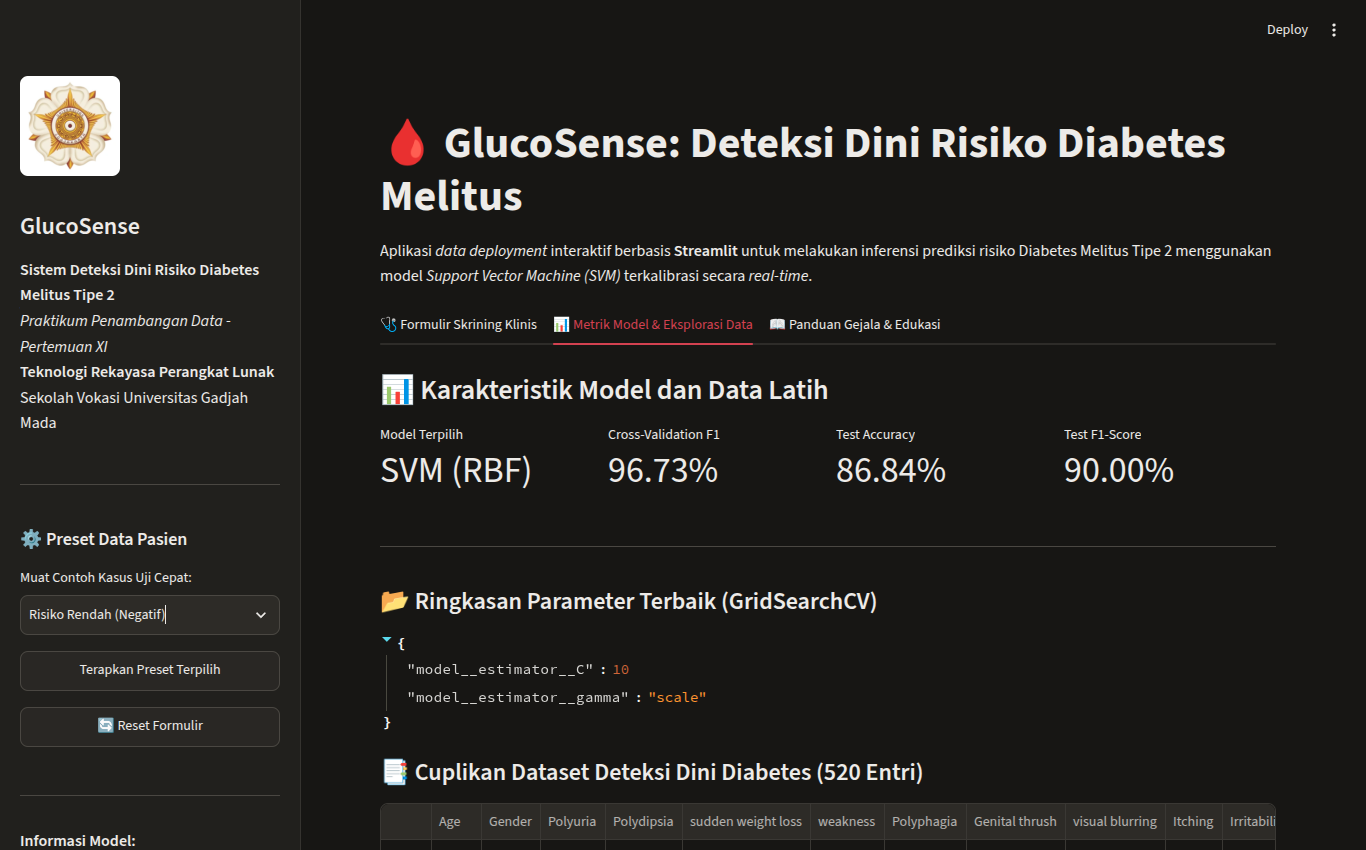
\includegraphics[width=0.88\textwidth]{images/streamlit-ss-08-antarmuka-glucosense-metrik-eksplorasi.png}
	\caption{Tampilan Metrik Evaluasi Model dan Eksplorasi Data Latih GlucoSense (Tab 2).}
	\label{fig:ss-s08}
\end{figure}

\begin{figure}[H]
	\centering
	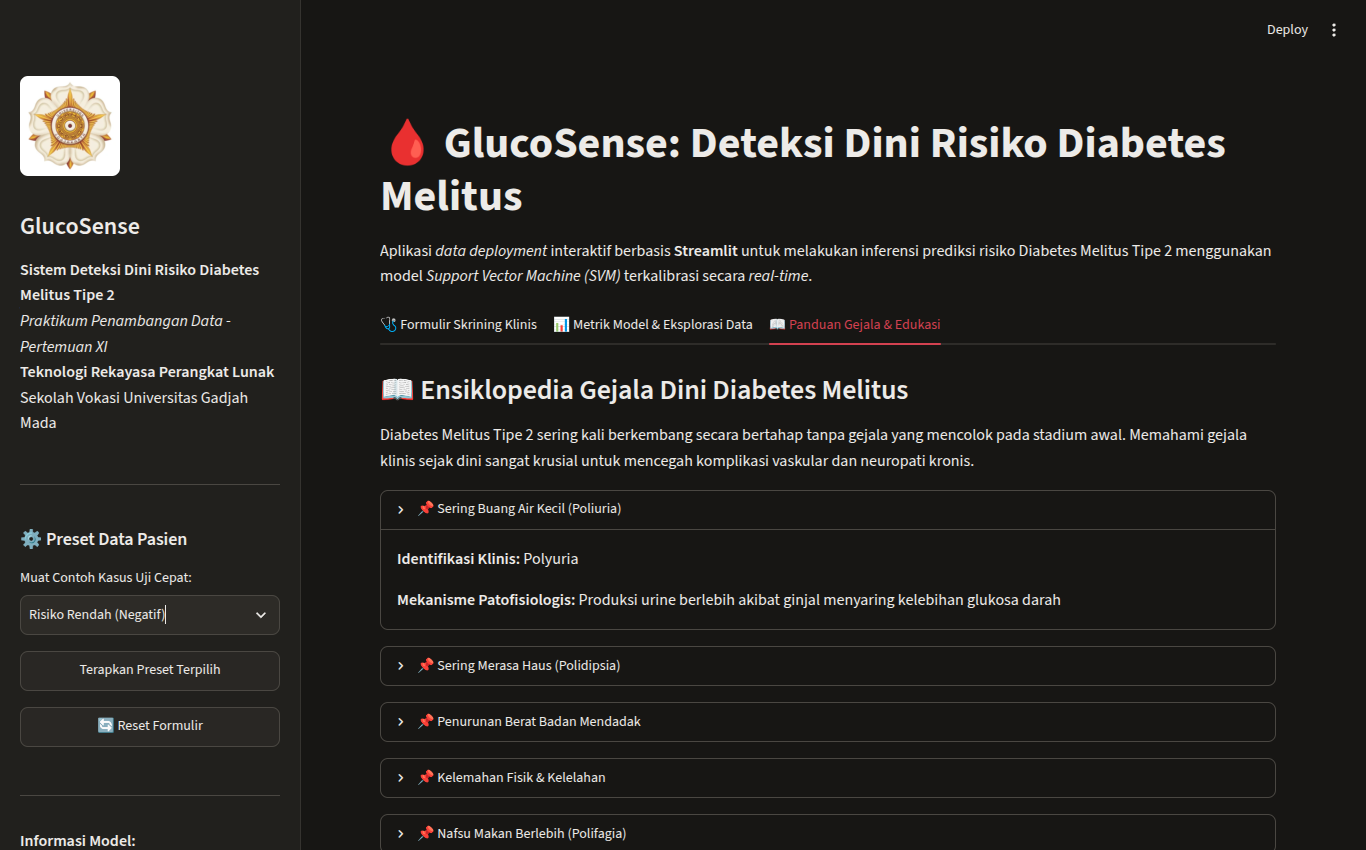
\includegraphics[width=0.88\textwidth]{images/streamlit-ss-09-antarmuka-glucosense-panduan-gejala.png}
	\caption{Ensiklopedia Panduan Gejala Klinis Diabetes Menggunakan st.expander (Tab 3).}
	\label{fig:ss-s09}
\end{figure}

\section{Analisis Komparatif Mendalam: Flask vs Streamlit}
Berdasarkan pengalaman langsung merancang dan menguji aplikasi \textit{web service} (Flask) serta \textit{data application} (Streamlit) pada proyek GlucoSense dan modul HCV, berikut analisis perbandingan teknis komprehensif kedua platform:

\subsection{Rekapitulasi Hasil Pengujian Skenario Klinis}
Sebagai pembuktian komparasi langsung kemampuan penyajian inferensi kedua kerangka kerja, pengujian skenario klinis pasien risiko tinggi, pasien risiko rendah, data HCV, dan penanganan galat masukan dijalankan pada kedua aplikasi. Hasil evaluasi komparatif dirangkum pada Tabel~\ref{tab:rekapitulasi-uji-klinis}.

\begin{table}[H]
\centering
\caption{Rekapitulasi Hasil Uji Kasus Klinis pada Implementasi Flask dan Streamlit.}
\label{tab:rekapitulasi-uji-klinis}
\small
\setlength{\tabcolsep}{3.5pt}
\begin{tabularx}{\linewidth}{|>{\raggedright\arraybackslash}p{2.6cm}|>{\raggedright\arraybackslash}X|>{\centering\arraybackslash}p{2.2cm}|>{\centering\arraybackslash}p{2.2cm}|>{\raggedright\arraybackslash}X|}
\hline
\textbf{Skenario Pasien} & \textbf{Gejala Masukan} & \textbf{Hasil Flask} & \textbf{Hasil Streamlit} & \textbf{Tindakan Medis} \\
\hline
Kasus Positif (GlucoSense) & Usia 55, Laki-laki, Poliuria (+), Polidipsia (+), Penurunan BB (+), Lemah (+), Polifagia (+) & Risiko Tinggi (Peluang 99,3\%) & Risiko Tinggi (Peluang 98,43\%) & Rujukan segera uji laboratorium HbA1c dan konsultasi dokter spesialis \\
\hline
Kasus Negatif (GlucoSense) & Usia 28, Perempuan, Asimtomatik (tanpa poliuria, polidipsia, kelemahan fisik) & Risiko Rendah (Peluang 0,1\%) & Risiko Rendah (Peluang 0,87\%) & Edukasi pola hidup sehat, olahraga rutin, dan pemantauan tahunan \\
\hline
Pasien Uji (Modul HCV) & AST 140,8, ALT 41,7, BIL 35,0, GGT 110,0, ALB 38,5, CHE 5,34 & Sirosis (\textit{Cirrhosis}) & Sirosis (\textit{Cirrhosis}) & Pemeriksaan USG abdomen, serologi, dan uji fungsi hati \\
\hline
Validasi Isian Tak Valid & Kolom usia dikosongkan atau diisi karakter non-angka & Ditolak: 400 Bad Request & Validasi Form Peringatan & Mencegah galat server dengan validasi tipe data \\
\hline
\end{tabularx}
\end{table}

\subsection{Kecepatan Pengembangan dan Kompleksitas Kode}
Streamlit menawarkan kecepatan perancangan antarmuka yang jauh lebih pesat (\textit{development velocity} tinggi). Untuk membangun form dengan 14 parameter gejala pada Flask, pengembang harus menuliskan rute backend Python, merancang berkas HTML Jinja2 (\texttt{index.html} dan \texttt{result.html}), mengatur stylesheet CSS untuk layout grid, serta menambahkan logika penanganan pesan galat. Sebaliknya, pada Streamlit, seluruh komponen antarmuka, tata letak kolom, grafik batang, metrik KPI, dan form input dapat diselesaikan murni dalam satu berkas skrip Python tunggal (\texttt{app.py}) sekitar 200 baris kode tanpa menyentuh HTML atau CSS.

\subsection{Karakteristik Arsitektur dan Efisiensi Sumber Daya}
Flask mengadopsi model \textit{stateless request-response} yang sangat efisien dalam konsumsi memori server. Ketika permintaan HTTP selesai ditangani, memori permintaan langsung dibebaskan oleh sistem. Model ini sangat tangguh untuk menangani ribuan permintaan konkuren tinggi via server WSGI produksi. Sebaliknya, Streamlit mengeksekusi ulang seluruh skrip pada setiap aksi pengguna (\textit{reactive script re-run}). Jika pengembang tidak memanfaatkan dekorator caching (\texttt{@st.cache\_resource} dan \texttt{@st.cache\_data}), pemuatan ulang model machine learning dan dataset akan menimbulkan \textit{overhead} komputasi tinggi dan memperlambat waktu respons aplikasi secara signifikan.

\subsection{Kesesuaian Skenario Penerapan Industri}
Kedua teknologi memiliki spesialisasi dan posisi yang saling melengkapi dalam ekosistem MLOps:
\begin{itemize}[noitemsep, topsep=2pt, parsep=1pt]
	\item \textbf{Gunakan Flask:} Jika tujuan deployment adalah menyediakan layanan \textit{Backend RESTful API} atau \textit{microservice} tanpa antarmuka grafis yang akan dikonsumsi oleh aplikasi klien lain (aplikasi seluler Android/iOS, aplikasi web React/Vue, perangkat Internet of Things, atau sistem perbankan/rumah sakit).
	\item \textbf{Gunakan Streamlit:} Jika tujuan deployment adalah membangun \textit{Rapid Prototyping}, dashboard analitik data internal, alat validasi model bagi \textit{domain expert} (dokter, analis risiko), demonstrasi portofolio data science, atau aplikasi bukti konsep (\textit{Proof of Concept}) dengan waktu rilis yang sangat cepat.
\end{itemize}

\clearpage

\chapter{Kesimpulan}
Berdasarkan seluruh tahapan percobaan modul dan tugas mandiri yang telah diselesaikan pada Pertemuan X dan XI mengenai *Model Deployment*, dapat ditarik beberapa kesimpulan penting:
\begin{enumerate}[noitemsep, topsep=2pt, parsep=1pt]
	\item \textit{Model deployment} merupakan fase krusial dalam siklus hidup machine learning yang mentransformasikan model statis hasil evaluasi menjadi layanan komputasi aktif yang dapat diakses pengguna melalui antarmuka web interaktif maupun REST API.
	\item Teknik serialisasi menggunakan pustaka \texttt{joblib.dump} berhasil menyimpan model \textit{Decision Tree} (5.785 byte) dan model \texttt{Pipeline} SVM GlucoSense (14 KB) ke dalam berkas biner. Pustaka \texttt{joblib.load} mampu memuat kembali objek model ke memori RAM tanpa kehilangan parameter atau performa inferensi.
	\item Penanganan dependensi versi pustaka dan urutan fitur masukan sangat menentukan keberhasilan deserialisasi. Penyesuaian tipe data label target menjadi bilangan bulat (\texttt{int}) berhasil mengatasi galat bawaan pada kode modul HCV.
	\item Model SVM RBF terkalibrasi yang dilatih untuk proyek kelompok GlucoSense menghasilkan performa yang andal dengan F1-score validasi silang 0,9673, akurasi uji 86,84\%, dan F1-score uji 90,00\%, serta mampu menghasilkan probabilitas risiko kontinu melalui kalibrasi penskalaan Platt.
	\item Implementasi Flask berhasil menyajikan layanan web service berbasis RESTful API ganda: antarmuka formulir HTML untuk pengguna umum dan endpoint \texttt{/api/predict} untuk integrasi sistem JSON via HTTP POST.
	\item Implementasi Streamlit berhasil menghadirkan dasbor analitik data yang sangat interaktif dan modern melalui modul multi-tab (\textit{screening}, eksplorasi data, dan panduan edukasi medis), dioptimalkan menggunakan dekorator \texttt{@st.cache\_resource} dan \texttt{st.session\_state}.
	\item Evaluasi komparatif menegaskan bahwa Streamlit unggul telak dalam kecepatan pengembangan (\textit{rapid prototyping}) dan dasbor data analitis, sedangkan Flask unggul dalam fleksibilitas arsitektur, efisiensi beban server, dan penyediaan backend RESTful API berskala produksi.
\end{enumerate}

\clearpage

%======================================================================
% DAFTAR PUSTAKA
%======================================================================
\begin{thebibliography}{99}
	\bibitem{repo-kode} H. R. Prasetya, ``Praktikum Penambangan Data: Model Deployment (Flask \& Streamlit),'' GitHub, 2026. [Online]. Tersedia: \url{https://github.com/hafidzrizqullahprasetya/PPD}.

	\bibitem{breiman1984} L. Breiman, J. H. Friedman, R. A. Olshen, dan C. J. Stone, \textit{Classification and Regression Trees}. Belmont, CA, USA: Wadsworth, 1984.

	\bibitem{cortes1995} C. Cortes dan V. Vapnik, ``Support-vector networks,'' \textit{Machine Learning}, vol. 20, no. 3, hlm. 273--297, 1995.

	\bibitem{fielding2000} R. T. Fielding, ``Architectural styles and the design of network-based software architectures,'' Ph.D. dissertation, University of California, Irvine, CA, USA, 2000.

	\bibitem{han2022} J. Han, J. Pei, dan H. Tong, \textit{Data Mining: Concepts and Techniques}, edisi ke-4. Cambridge, MA, USA: Morgan Kaufmann, 2022.

	\bibitem{islam2020} M. M. F. Islam, R. Ferdousi, S. Rahman, dan H. Y. Bushra, ``Likelihood prediction of diabetes at early stage using data mining techniques,'' dalam \textit{Computer Vision and Machine Intelligence in Medical Image Analysis}. Singapore: Springer, 2020, hlm. 113--125.

	\bibitem{joblib-persistence} Joblib developers, ``Persistence,'' Joblib Documentation, 2024. [Online]. Tersedia: \url{https://joblib.readthedocs.io/en/stable/user_guide/persistence.html}.

	\bibitem{uci-hcv} R. Lichtinghagen, F. Klawonn, dan G. Hoffmann, ``HCV data,'' UCI Machine Learning Repository, 2020. [Online]. Tersedia: \url{https://doi.org/10.24432/C5D612}.

	\bibitem{flask-quickstart} Pallets, ``Quickstart,'' Flask Documentation, 2024. [Online]. Tersedia: \url{https://flask.palletsprojects.com/en/stable/quickstart/}.

	\bibitem{flask-deploy} Pallets, ``Deploying to production,'' Flask Documentation, 2024. [Online]. Tersedia: \url{https://flask.palletsprojects.com/en/stable/deploying/}.

	\bibitem{sklearn2011} F. Pedregosa \textit{et al.}, ``Scikit-learn: Machine learning in Python,'' \textit{Journal of Machine Learning Research}, vol. 12, hlm. 2825--2830, 2011.

	\bibitem{platt1999} J. C. Platt, ``Probabilistic outputs for support vector machines and comparisons to regularized likelihood methods,'' dalam \textit{Advances in Large Margin Classifiers}. Cambridge, MA, USA: MIT Press, 1999, hlm. 61--74.

	\bibitem{sklearn-persistence} Scikit-learn developers, ``Model persistence,'' Scikit-learn Documentation, 2024. [Online]. Tersedia: \url{https://scikit-learn.org/stable/model_persistence.html}.

	\bibitem{sklearn-calibration} Scikit-learn developers, ``Probability calibration,'' Scikit-learn Documentation, 2024. [Online]. Tersedia: \url{https://scikit-learn.org/stable/modules/calibration.html}.

	\bibitem{streamlit-docs} Streamlit Inc., ``Streamlit Documentation,'' 2024. [Online]. Tersedia: \url{https://docs.streamlit.io/}.

	\bibitem{streamlit-caching} Streamlit Inc., ``Caching in Streamlit,'' 2024. [Online]. Tersedia: \url{https://docs.streamlit.io/develop/concepts/architecture/caching}.

	\bibitem{treveil2020} M. Treveil \textit{et al.}, \textit{Introducing MLOps: How to Scale Machine Learning in the Enterprise}. Sebastopol, CA, USA: O'Reilly Media, 2020.

	\bibitem{uci-diabetes} UCI Machine Learning Repository, ``Early stage diabetes risk prediction dataset,'' 2020. [Online]. Tersedia: \url{https://doi.org/10.24432/C5VG8H}.
\end{thebibliography}

\end{document}
